\documentclass[titlepage=true, parskip=full]{scrartcl}
\usepackage[utf8]{inputenc} % use utf8 file encoding for TeX sources
\usepackage[T1]{fontenc}    % avoid garbled Unicode text in pdf
\usepackage{palatino}	      % because "Computer Modern" standard font is illegible
\usepackage{mathpazo}
\usepackage{amsmath}
\usepackage[ngerman]{babel}  % german hyphenation, quotes, etc
\usepackage{hyperref}       % detailed hyperlink/pdf configuration
\hypersetup{                % ‘texdoc hyperref‘ for options
	pdftitle={PSE: Implementierungsbericht},%
	bookmarks=true,%
}
\usepackage{graphicx}       % provides commands for including figures
\usepackage{csquotes}       % provides \enquote{} macro for "quotes"
\usepackage[nonumberlist, numberedsection]{glossaries}     % provides glossary commands
\usepackage{enumitem}
\usepackage{tikz}
\usepackage{tikz-uml}
\usepackage{tikz-er2}
\usepackage{comment}
\usepackage{array}
\usepackage{longtable}
\usepackage{hhline}
\usepackage{placeins}
\usepackage{needspace}
\usepackage[toc, page]{appendix}
\usepackage{tabularx}
\usepackage{tabulary}
\usepackage{multirow}
\usepackage{multicol}
\usepackage{rotating}
\usepackage{microtype}
\usepackage{MnSymbol}
\usetikzlibrary{positioning}
\usepackage{pgfgantt}
\usepackage{float}
\usepackage{listings}
\usepackage{xcolor}

\colorlet{punct}{red!60!black}
\definecolor{background}{HTML}{EEEEEE}
\definecolor{delim}{RGB}{20,105,176}
\colorlet{numb}{magenta!60!black}

% Kommandos für Atomare und JSON-Werte:
\newcommand{\jsonatom}[1]{$\langle\textnormal{\textit{#1}}\rangle$}
\newcommand{\jsonobj}[1]{$\llangle\textnormal{\textit{#1}}\rrangle$}
\newcommand{\jsonpart}[2]{$\llangle\textnormal{\textit{#1}\,[#2]}\rrangle$}

\lstdefinelanguage{json}{
    basicstyle=\normalfont\ttfamily,
    numbers=left,
    numberstyle=\scriptsize,
    escapeinside={(*}{*)},
    stepnumber=1,
    numbersep=8pt,
    showstringspaces=false,
    breaklines=true,
    frame=lines,
    backgroundcolor=\color{background},
    literate=
     *{0}{{{\color{numb}0}}}{1}
      {1}{{{\color{numb}1}}}{1}
      {2}{{{\color{numb}2}}}{1}
      {3}{{{\color{numb}3}}}{1}
      {4}{{{\color{numb}4}}}{1}
      {5}{{{\color{numb}5}}}{1}
      {6}{{{\color{numb}6}}}{1}
      {7}{{{\color{numb}7}}}{1}
      {8}{{{\color{numb}8}}}{1}
      {9}{{{\color{numb}9}}}{1}
      {:}{{{\color{punct}{:}}}}{1}
      {,}{{{\color{punct}{,}}}}{1}
      {\{}{{{\color{delim}{\{}}}}{1}
      {\}}{{{\color{delim}{\}}}}}{1}
      {[}{{{\color{delim}{[}}}}{1}
      {]}{{{\color{delim}{]}}}}{1},
}


%\usepackage[vlined]{algorithm2e}
% see http://ctan.math.utah.edu/ctan/tex-archive/macros/latex/contrib/algorithm2e/doc/algorithm2e.pdf  for more information
\DontPrintSemicolon
\SetKwSwitch{Switch}{Case}{Other}{case}{of}{}{else}{}{}
\SetKw{KwAssert}{assert}
\SetKw{KwInvariant}{invariant}
\SetKw{KwStep}{step}
\SetKw{KwDownto}{downto}	
\SetKw{KwArrayOf}{array of }
\SetKw{KwArray}{array }
\SetKw{KwOf}{ of }
\SetKw{KwNot}{ not }
\SetKw{KwIs}{ is }
\SetKw{KwAnd}{ and }
\SetKw{KwOr}{ or }
\SetKw{KwBreak}{break}
\SetKw{KwThrow}{throw}
\SetKw{KwTrue}{true}
\SetKw{KwFalse}{false}
\SetKwBlock{KwFunc}{function}{}
\SetKwBlock{KwProc}{procedure}{}
\newcommand{\Function}[2]{\KwFunc({#1}){#2}}
\newcommand{\Procedure}[2]{\KwProc({#1}){#2}}
\SetKwData{KwList}{List}
\SetKwData{KwSet}{Set}
\newcommand{\KwListOf}{\KwList \KwOf}
\newcommand{\KwSetOf}{\KwSet \KwOf}
\SetKwComment{Comment}{// }{}
\newcommand{\LComment}[1]{\hspace{-2pt}\Comment*[l]{#1}}
\newcommand{\RComment}[1]{$ \qquad $ \Comment*[h]{#1} \\}
\newcommand{\RCommentNoBreak}[1]{$ \qquad $ \Comment*[h]{#1}}
\newcommand{\MyCommentSty}[1]{\emph{\textcolor{gray}{#1}}}
\SetCommentSty{MyCommentSty}
\SetFuncSty{emph}
\definecolor{kwblue}{rgb}{0.3,0.3,1}
\newcommand{\MyKwSty}[1]{\textcolor{kwblue}{\textbf{#1}}}
\SetKwSty{MyKwSty}
\newcommand{\Call}[2]{\FuncSty{#1}(#2)}
\newcommand{\pluseq}{\mathrel{+}=}
\newcommand{\Var}[1]{\textit{#1}}

% needed to define linebreak points without hyphenation (useful for URL wrapping)
\newcommand{\+}{\discretionary{}{}{}}

\renewcommand{\arraystretch}{1.24}  % for proper row spacing in tables

%%%%%%%%%%%%%%%%%%%%%%%%%%%
% longtable multirow page break insanity fix – http://tex.stackexchange.com/a/52101
\makeatletter
\def\@cline#1-#2\@nil{%
	\omit
	\@multicnt#1%
	\advance\@multispan\m@ne
	\ifnum\@multicnt=\@ne\@firstofone{&\omit}\fi
	\@multicnt#2%
	\advance\@multicnt-#1%
	\advance\@multispan\@ne
	\leaders\hrule\@height\arrayrulewidth\hfill
	\cr
	\noalign{\nobreak\vskip-\arrayrulewidth}}
\makeatother
%%%%%%%%%%%%%%%%%%%%%%%%%%%

% For Christ's sake, I'm sick and tired of this f*cking orphan/widow crap!
\widowpenalty=10000
\clubpenalty=10000
% Source: somewhere on tex.stackexchange.com

\renewcommand{\to}{\longrightarrow} % proper math typography
\newcommand{\NN}{\mathbb{N}}
\newcommand{\RR}{\mathbb{R}}
\newcommand{\QQ}{\mathbb{Q}}

\addto\captionsngerman{\let\appendixtocname\appendixname\let\appendixpagename\appendixname}

% fix hyphenation
\hyphenation{Log-out Log-in Ak-tions Ak-tion ge-öff-net liken dis-liken Like Dis-like No-ti-fi-ca-tion Mo-dule inkl Au-tho-ri-za-tion Web-App Ar-chi-tek-tur-en Ge-ne-rie-rungs Stu-di-en-plan Client}

\usepackage{enumitem}
\setlist[itemize]{nosep}
\shorthandon{"}
%\makeglossaries
%%
% % Automatisch generiertes Glossar
%
%\glsaddall % das sorgt dafür, dass alles Glossareinträge gedruckt werden, nicht nur die verwendeten. Das sollte nicht nötig sein!
%
% % Glossareinträge
%
\newglossaryentry{Rest}
{
	name=REST,
	description={Abk. für Representational State Transfer, Programmierparadigma für \glspl{Webservice} auf Basis des HTTP-Protokolls}
}

\newglossaryentry{ECTS-Punkte}
{
	name=ECTS-Punkte,
	description={Leistungspunkte, die für ein erfolgreich absolviertes \gls{Modul} von der Hochschule auf Basis des ECTS-Punktesystems vergibt werden, und mit denen der Arbeitsaufwand gemessen wird},
}

\newglossaryentry{Generierungs-Tool}
{
	name=Generierungs-Tool,
	description={Tool, für die automatische Erstellung bzw. Vervollständigung von Studienpläne},
}


\newglossaryentry{Webservice}
{
	name=Webservice,
	plural=Webservices,
	description={Softwareanwendung, die über ein Netzwerk bereitgestellt wird}
}

\newglossaryentry{Plug-In-Paket}
{
	name=Plug-In-Paket,
	plural=Plug-In-Pakete,
	description={Paket bestehend aus mehreren \glspl{Plug-In}}
}

\newglossaryentry{iMage}
{
	name={iMage},
	description={Bildbearbeitungssoftware der Firma SWT. Bietet im Basispaket nur Funktionalitäten zur Skalierung und Drehung von Bildern}
}

\newglossaryentry{Internetbrowser}
{
	name={Internetbrowser},
	description={Programm, mit dem Websites gefunden, gelesen und verwaltet werden können, mit aktiviertem JavaScript}
}

\newglossaryentry{Online-Shop}
{
	name={Online-Shop},
	description={Internetseite, die Produkte zum Kauf anbietet}
}

\newglossaryentry{KIT}
{
	name=KIT,
	description={Das Karlsruher Institut für Technologie ist die Forschungsuniversität in der Helmholtz-Gemeinschaft. Standort der Universität ist Karlsruhe. }
}

\newglossaryentry{SCC}
{
	name=SCC,
	plural=SCC,
	description={Das Steinbuch Center for Computing ist ein Institut und das zentrale Rechenzentrum des \gls{KIT}s.}
}

\newglossaryentry{Benutzer}
{
	name=Benutzer,
	plural=Benutzer,
	description={Ein am \gls{KIT} eingeschriebener Student, der über ein gültigen Account beim \gls{SCC} verfügt.}
}

\newglossaryentry{Wizard}
{
	name=Wizard,
	plural=Wizards,
	description={Ein Wizard ist ein Subsystem, welches einen \gls{Benutzer} visuell durch eine Systemfunktionalität führt und dabei vom \gls{Benutzer} bestimmte Interaktionen mit dem System fordert.}
}

\newglossaryentry{Drag-and-Drop}
{
	name=Drag-and-Drop,
	description={(deutsch: "Ziehen und Ablegen") Eine Methode zur Bedienung grafischer Benutzeroberflächen bei der grafische Elemente mittels eines Mauszeigers bewegt werden.}
}

\newglossaryentry{Shibboleth Identity Provider}
{
	name=Shibboleth Identity Provider,
	description={Ein genau spezifiziertes System zum Login mittels einer von einer dritten Instanz bereitgestellten Identität.}
}

\newglossaryentry{Studiengang}
{
	name=Studiengang,
	description={Ein vom KIT angebotener, auf einer Studien- und Prüfungsordnung und einem Modulhandbuch basierender Studiengang.}
}

\newglossaryentry{Semester des Studienbeginns}
{
	name=Semester des Studienbeginns,
	description={Das Semester in welchem der \gls{Benutzer} im ersten Fachsemester des \gls{Studiengang}s war.}
}

\newglossaryentry{Modul}
{
	name=Modul,
	plural=Module,
	description={Ein Modul ist ein Teilblock des Studiums, welcher aus verschiedenartigen Veranstaltungen (genannt \glspl{Teilmodul}) bestehen kann und für welchen man nach Ablegung eventueller \glspl{Modulpruefung} eine festgelegte Anzahl an ECTS-Punkten erhält.}
}
\newglossaryentry{Teilmodul}
{
	name=Teilmodul,
	plural=Teilmodule,
	description={Ein Teilmodul ist eine universitäre Veranstaltung, welche als Teil eines Moduls besucht werden kann und mittels einer (wie auch immer gearteten) \gls{Modulpruefung} bestanden werden kann.}
}
\newglossaryentry{Modulpruefung}
{
	name=Modulprüfung,
	plural=Modulprüfungen,
	description={Eine Modulprüfung ist eine Prüfung, welche abgelegt werden muss um ein Modul \glslink{Modul abgeschlossen}{abzuschließen}.}
}
\newglossaryentry{Zur Pruefung angetreten}
{
	name=Zur Pruefung angetreten,
	description={Ein \gls{Benutzer} ist zu einer \gls{Modulpruefung} angetreten, wenn er sich fristgerecht für selbige angemeldet und nicht fristgerecht abgemeldet hat.}
}

\newglossaryentry{Modul abgeschlossen}
{
	name=Modul abgeschlossen,
	description={Ein \gls{Modul} gilt als abgeschlossen, wenn der \gls{Benutzer} alle nach Modulhandbuch notwendigen \glspl{Modulpruefung} bestanden hat.}
}

\newglossaryentry{Modul begonnen}
{
	name=Modul begonnen,
	description={Ein \gls{Modul} gilt als begonnen, wenn der \gls{Benutzer} zu mindestens einer \gls{Modulpruefung} \glslink{Zur Pruefung angetreten}{angetreten} ist.}
}

\newglossaryentry{Studienplan}
{
	name=Studienplan,
	plural=Studienpläne,
	description={Eine Zusammenstellung von Modulen, in welcher enthalten ist wann welches Modul planmäßig \glslink{Modul begonnen}{begonnen} werden soll.}
}
\shorthandoff{"}

\begin{document}
	
\begin{titlepage}
	\centering
	{\huge \bfseries \sffamily Studienplanung als Generierung von Workflows mit Compliance-Anforderungen: Planerstellung und Visualisierung\par}
	\vspace{1cm}
	{\LARGE Implementierungsbericht\par}
	\vfill
	\begin{tabular}{>{\Large}c}
		Nada Chatti\\
		Daniel Jungkind\\
		Hannes Kuchelmeister\\
		Ulrike Rheinheimer\\
		Paul Samuel M. Teuber\\
		\textbf{Tim Niklas Uhl}
	\end{tabular}
	\vfill
	15. Februar 2017
\end{titlepage}
\tableofcontents
\pagebreak

%
% % Hier beginnt die Gliederung des Pflichtenhefts
\section{Einleitung}
Der Implementierungsbericht des Projekts „Studienplanung als Generierung von Workflows mit Compliance-Anforderungen: Planerstellung und Visualisierung“ beschreibt die Umsetzung des zuvor im Pflichtenheft und Entwurf spezifizierten Projekts. In über ????? Zeilen Java-, Javascript-, HTML- und CSS-Code liegt jetzt eine fertige, nur noch zu optimierende Anwendung vor. In diesem Bericht möchten wir dabei auf implementierte und ausgelassen Features eingehen, Änderungen beschreiben und begründen, und die Implementierungsphase (einschließlich aller durchgemachten Nächte) reflektieren.
Zusammenfassend ist dieser Bericht Ende einer arbeitsintensiven, aber erfolreichen Phase, die als Endprojekt ein einmalig sinnvolles, dringendnotweniges und jedem Studenten zu empfehlendes Studienplanungshilfsmittel zur Verfügung stellt.




\FloatBarrier
\section{Änderungen am Entwurf}

\FloatBarrier
\subsection{Änderungen an der Datenbasis}
\label{subsec:changes_database}

Um die gestellte Moduldatenbank in unseren Entwurf zu integrieren, haben wir diese um \textit{Fields} (Bereiche) und \textit{Rule-Groups} erweitert.

\textit{Fields} modellieren Bereiche eines Studiengangs. Zu jedem Bereich gehören eine Mindestanzahl an ECTS, die in diesem Bereich belegt werden muss. Ist das Attribut \textit{choosable} gesetzt, so verfügt ein Bereich auch über Vertiefungsfächer. Damit kann der Benutzer bei der Generierung in jedem auswählbaren Bereich ein Vertiefungsfach angeben, aus welchem der Generierer bevorzugt Module wählen soll. Diese Änderung sorgt unter anderem dafür, dass die nötigen 180~ECTS für den Bachelor"=Abschluss nicht hartkodiert werden müssen, sondern aus der Summe der ECTS der zu einem Studiengang gehörigen Bereiche berechnet werden können.

\textit{Rule-Groups} beschreiben Gruppen von Modulen, die bezüglich der  Modulanzahl beschränkt sind. Das heißt, dass innerhalb einer Gruppe eine Mindest- und eine Maximalanzahl an Modulen vorgeschrieben ist, um ein Studienfach erfolgreich abschließen zu können. Dies stellt zum Beispiel sicher, dass mindestens zwei Stammmodule sowie ein Proseminar belegt werden.

Diese Änderungen ermöglichen eine stärkere Abstraktion der Bedingungen eines Studiengangs, was die Modellierung von unterschiedlichen Studiengängen vereinfacht.

\begin{figure}
	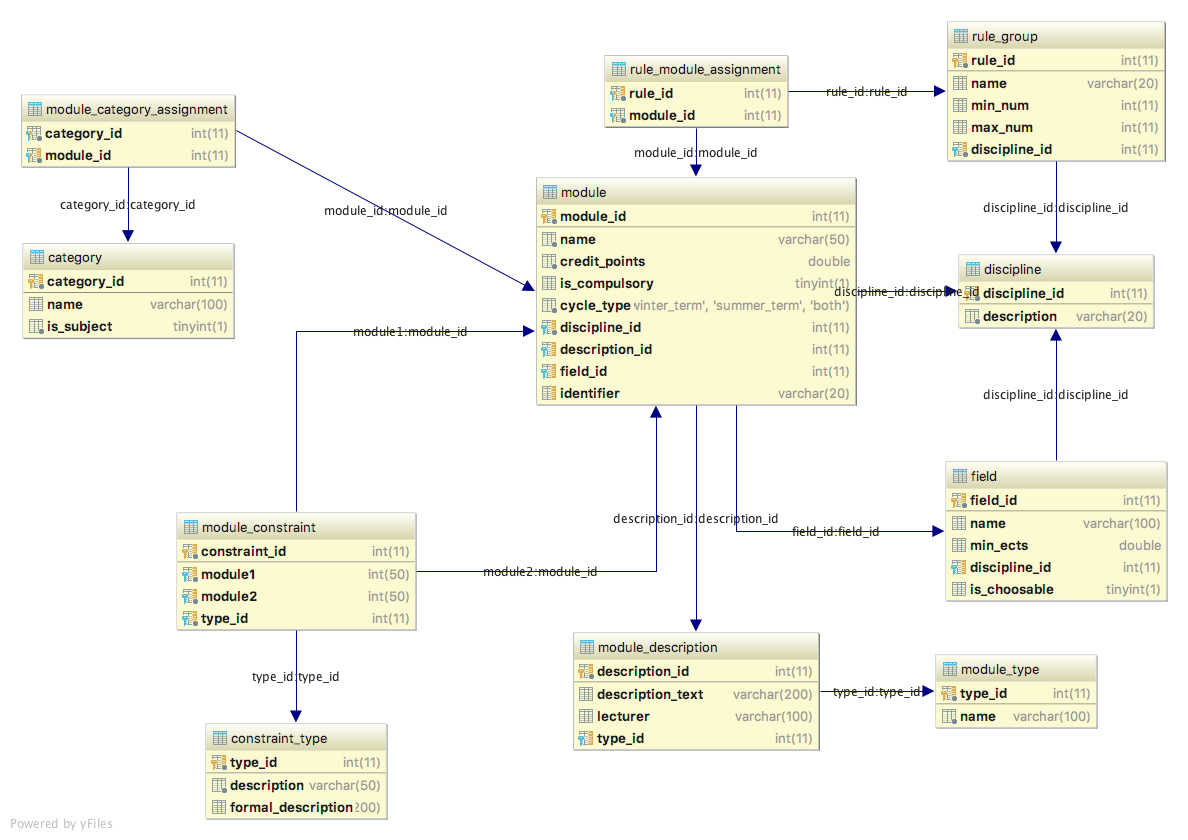
\includegraphics[width = \textwidth]{diagrams/module_diagram.png}
	\caption{Übersicht über die Struktur der Moduldatenbank}
\end{figure}

\FloatBarrier
\subsection{Änderungen an der REST-Schnittstelle}
\label{subsec:changes_rest}

Nachfolgend eine Auflistung aller atomaren Werte und JSON"=Datenklassen, deren Definitionen sich geändert haben.

\subsubsection*{JSON-Atome}

\begin{longtable}{p{.22\linewidth} p{.73\linewidth}}
	Bezeichner
	& Erklärung \\
	\hline
	\endfirsthead
	
	Bezeichner
	& Erklärung \\
	\hline 
	\endhead
	
	\hline
	\endlastfoot
	
	\lbljsonatom{Modul-Turnus} 
	& $ \in \{\verb|"WT"|, \verb|"ST"|, \verb|"both"|\}$. \\
	\lbljsonatom{Semester-Typ} 
	& $ \in \{\verb|"WT"|, \verb|"ST"|\}$. \\
	\lbljsonatom{Semester-Zahl}
	& Zahl des aktuellen Semesters des Benutzers. \\
	\lbljsonatom{Filter-URI-Identifier}
	& String, mit welchem der Filter in GET-Parametern identifiziert wird. \\

\end{longtable}

\subsubsection*{JSON-Datenklassen}

\begin{lstlisting}[language=json]
(*\lbljsonobj{Student}*) = {
	"discipline": (*\jsonpart{Studienfach}{id}*),
	"study-start": (*\jsonobj{Studienbeginn}*),
	"passed-modules": (*\jsonlist{\jsonpart{Modul}{id, name, creditpoints, lecturer, semester}}*),
	"current-semester": (*\jsonatom{Semester-Zahl}*)
}
\end{lstlisting}

\begin{lstlisting}[language=json]
(*\lbljsonobj{Modul}*) = {
	"id": (*\jsonatom{Modul-ID}*),
	"name": (*\jsonatom{Modul-Name}*),
	"categories" : (*\jsonlist{\jsonobj{Kategorie}}*),
	"semester": (*\jsonatom{Modul-Semester}*),
	"cycle-type": (*\jsonatom{Modul-Turnus}*),
	"creditpoints": (*\jsonatom{Modul-Creditpoints}*),
	"lecturer": (*\jsonatom{Modul-Dozent}*),
	"preference": (*\jsonatom{Modul-Präferenz}*),
	"compulsory": (*$\langle$*)true(*$\vert$*)false(*$\rangle$*),
	"description": (*\jsonatom{Modul-Beschreibung}*),	
	"constraints": (*\jsonlist{\jsonobj{Constraint}}*)
}
\end{lstlisting}

\begin{lstlisting}[language=json]
(*\lbljsonobj{Filter}*) = {
	"id": (*\jsonatom{Filter-ID}*),
	"name": (*\jsonatom{Filter-Name}*),
	"uri-name": (*\jsonatom{Filter-URI-Identifier}*),
	"default-value": (*\jsonatom{Filter-Default}*),
	"tooltip": (*\jsonatom{Filter-Tooltip}*),
	"specification": (*\jsonobj{Filter-Eigenschaften}*)
}
\end{lstlisting}


\begin{lstlisting}[language=json]
(*\lbljsonobj{Studienplan}*) = {
	"id": (*\jsonatom{Studienplan-ID}*),
	"status": (*\jsonatom{Studienplan-Status}*),
	"creditpoints-sum": (*\jsonatom{Studienplan-Gesamt-Creditpoints}*),
	"name": (*\jsonatom{Studienplan-Name}*),
	"modules": (*\jsonlist{\jsonpart{Modul}{id, name, semester, creditpoints, cycle-type, lecturer, preference}}*),
	"violations": (*\jsonlist{\jsonobj{Constraint}}*),
	"field-violations": (*\jsonlist{\jsonpart{Field}{name, min-ects}}*),
	"rule-group-violations": (*\jsonlist{\jsonobj{Rule-Group}}*),
	"compulsory-violations": (*\jsonlist{\jsonpart{Modul}{name}}*)
}
\end{lstlisting}

\begin{lstlisting}[language=json]
(*\lbljsonobj{Field}*) = {
	"id": (*\jsonatom{Field-ID}*),
	"name": (*\jsonatom{Field-Name}*),
	"min-ects": (*\jsonatom{Field-Mindest-ECTS}*),
	"categories": (*\jsonlist{\jsonobj{Kategorie}}*),
}
\end{lstlisting}

\begin{lstlisting}[language=json]
(*\lbljsonobj{Rule-Group}*) = {
	"name": (*\jsonatom{Rule-Group-Name}*),
	"min-num": (*\jsonatom{Rule-Group-Modul-Mindestanzahl}*),
	"max-num": (*\jsonatom{Rule-Group-Modul-Höchstanzahl}*)
}
\end{lstlisting}

\begin{json}
(*\lbljsonobj{ModulesResult}*) = {
	"modules": (*\jsonlist{\jsonpart{Modul}{id, name, creditpoints, lecturer, cycle-type}}*)
}	
\end{json}

\begin{json}
(*\lbljsonobj{ModuleResult}*) = {
	"module": (*\jsonpart{Modul}{id, name, categories, cycle-type,  creditpoints, lecturer, compulsory, description, constraints}*)
}	
\end{json}

\begin{json}
(*\lbljsonobj{StudentPutRequest}*) = {
	"student": (*\jsonpart{Student}{discipline, study-start, passed-modules}*)
}	
\end{json}

\begin{json}
(*\lbljsonobj{PlanResult}*) = {
	"plan": (*\jsonpart{Studienplan}{id, name, status, creditpoints-sum, modules}*)
}	
\end{json}

\begin{json}
(*\lbljsonobj{PlanPutRequest}*) = {
	"plan": (*\jsonpart{Studienplan}{id, name, modules[id, semester]}*)
}	
\end{json}

\begin{json}
(*\lbljsonobj{PlanPutResult}*) = {
	"plan": (*\jsonpart{Studienplan}{id, name, modules[id, semester], status}*)
}	
\end{json}


\begin{json}
(*\lbljsonobj{PlanModulesResult}*) = {
	"modules": (*\jsonlist{\jsonpart{Modul}{id, name, creditpoints, lecturer, cycle-type, preference}}*)
}	
\end{json}

\begin{json}
(*\lbljsonobj{PlanModuleResult}*) = {
	"module": (*\jsonpart{Modul}{id, name, categories, cycle-type, creditpoints, lecturer, preference, compulsory, description, constraints}*)
}
\end{json}

\begin{json}
(*\lbljsonobj{PlanVerificationResult}*) = {
	"plan": (*\jsonpart{Studienplan}{id, status, violations, field-violations, rule-group-violations, compulsory-violations}*)
}
\end{json}

\begin{json}
(*\lbljsonobj{PlanProposalResult}*) = {
	"plan": (*\jsonpart{Studienplan}{status, modules}*)
}
\end{json}

\begin{json}
(*\lbljsonobj{FieldsResult}*) = {
	"fields": (*\jsonlist{\jsonobj{Field}}*)
}
\end{json}
\subsubsection*{REST-Zugriffsstruktur}

Hinzugefügt:
\begin{longtable}{| >{\hspace{0pt}} p{.11\textwidth} | >{\hspace{0pt}} p{.17\textwidth} | >{\hspace{0pt}} p{.28\textwidth} | >{\hspace{0pt}} p{.34\textwidth} |}
	\hline
	\textbf{Methode} & \textbf{URI} & \textbf{Beschreibung} & \textbf{Anfrage-Parameter\+/Rückgabewerte} \\ 
	\hhline{|=|=|=|=|}  
	\endfirsthead
	
	\hline
	\textbf{Methode} & \textbf{URI} & \textbf{Beschreibung} & \textbf{Anfrage-Parameter\+/Rückgabewerte} \\ 
	\hline  
	\endhead
	
	\hhline{|=|=|=|=|}   
	\endlastfoot
	%===============================================================================================
	GET & / & Abfrage, ob der REST-Service antwortet & Anfrage: --- \newline Rückgabe: --- (200 OK) \\
	\hhline{|=|=|=|=|} 
	GET & /fields & Gibt alle Bereiche des zum Studenten gehörenden Studiengangs zurück & Anfrage: --- \newline Rückgabe: \jsonobj{FieldsResult} 
\end{longtable}

Entfernt:
\begin{itemize}
	\item POST /plans/\jsonatom{Plan-ID} \quad (Plan duplizieren): \newline
		  Kann mit DELETE, POST und PUT erreicht werden (dabei geht aber der Verifikationsstatus verloren, s.u.).
	\item GET /subjects: \newline
		  Rückgabe in GET /fields verfügbar.
\end{itemize}

Geändert:
\begin{itemize}
	\item GET /modules: \quad \jsonobj{ModulesResult} geändert (s.o.)
	\item GET /modules/\jsonatom{Module-ID}: \quad \jsonobj{ModuleResult} geändert (s.o.)
	\item PUT /plans/\jsonatom{Plan-ID} \quad (Plan ersetzen): \newline
		  Nimmt jetzt nur noch Namen und Modulbelegung entgegen, der Verifikationsstatus wird auf „nicht verifiziert“ gesetzt. \newline
		  Anfrage: \jsonobj{PlanPutRequest} (geändert, s.o.) \newline
		  Rückgabe: \jsonobj{PlanPutResult} (geändert, s.o.)
	\item GET /plans/\jsonatom{Plan-ID}: \quad \jsonobj{PlanResult} geändert (s.o.)
	\item GET /plans/\jsonatom{Plan-ID}/modules: \quad \jsonobj{PlanModulesResult} geändert (s.o.)
	\item GET /plans/\jsonatom{Plan-ID}/modules/\jsonatom{Modul-ID}: \quad \jsonobj{PlanModuleResult} geändert (s.o.)
	\item GET /plans/\jsonatom{Plan-ID}/verification: \quad \jsonobj{PlanVerificationResult} geändert (s.o.)
	\item GET /plans/\jsonatom{Plan-ID}/proposal/\jsonatom{Zielfunktion-ID}: \newline
		  Da sich die Modellierung der Vertiefungsfächer geändert hat (siehe Kap.~\ref{subsec:changes_database}), werden auch die GET-Parameter wie folgt angepasst: \newline
		  Anfrage-Parameter: 
		  \subitem max-semester-ects=\jsonatom{Semester-ECTS-Maximum} 
		  \subitem fields=\jsonatom{Field-ID},...,\jsonatom{Field-ID}  
		  \subsubitem (Auflistung gewählter Bereiche) 
		  \subitem field-$k$=\jsonatom{Vertiefungsfach-ID} 
		  \subsubitem (für jeden gewählten Bereich mit ID $k$) \newline
		  Rückgabe: \jsonobj{PlanProposalResult} (geändert, s.o.)
	\item GET /plans/\jsonatom{Plan-ID}/pdf: \newline
		  Zurückgeschickt wird ein Dokument vom Typ ``text/html''. Der Nutzer kann dieses entweder manuell in ein PDF umwandeln (von gängigen Browsern unterstützt) oder direkt ausdrucken.
	\item PUT /student: \newline
		  Beim Ersetzen der Studenteninformationen werden die bestandenen Module aus allen Plänen gelöscht, in denen sie vorkommen. Alle Pläne werden weiterhin als „nicht verifiziert“ markiert. \newline
		  Anfrage: \jsonobj{StudentPutRequest} (geändert, s.o.) 
	\item GET /student: \newline
		  Es wird zusätzlich die \jsonatom{Semester-Zahl} zurückgeschickt (s. \jsonobj{Student}, geändert)
\end{itemize}




\FloatBarrier
\subsection{Client-Änderungen}

In der gesamten Client-Implementierung wurden Attributnamen den JSON-Definitionen angepasst, um die Standard-parse- und toJSON-Methoden nutzen zu können und Übersichtlichkeit durch Einheitlichkeit herzustellen.

\subsubsection{View-Paket}
\input{content/changes/client/client/view/subview.tex}
\input{content/changes/client/client/view/components/filter.tex}
\input{content/changes/client/client/view/components/uielement.tex}
\input{content/changes/client/client/view/components/uipanel.tex}


\subsubsection{Storage-Paket}
\input{content/changes/client/client/storage.tex}
\subsubsection{Router-Paket}
\input{content/changes/client/client/router.tex}

\subsubsection{Model-Paket}
\input{content/changes/client/client/model/module.tex}
\input{content/changes/client/client/model/plans.tex}
\input{content/changes/client/client/model/system.tex}
\input{content/changes/client/client/model/user.tex}






\FloatBarrier
\subsection{Server-Änderungen}

\subsubsection{Model-Paket}

\paragraph{Paket moduledata.*} Es wurden die Klassen Field und RuleGroup hinzugefügt, um die Modelländerungen abzubilden. Im ModuleDao-Interface wurden einige Bequemlichkeitsmethoden zum Finden von Kategorien, Bereichen, Vertiefungsfächern u. ä. hinzugefügt. Eine ConditionQueryConverter-Klasse unterstützt nun die Umwandlung von Condition-Objekten in SQL"=Statements, die dann mit Hibernate an die Datenbank geschickt werden können.



\subsubsection{Filter-Paket}
\label{subsubsec:filter}

Das Filter-Paket wurde grundlegend umgestaltet: Ein Filter enthält mittlerweile nur die Daten, die zum Filtern benötigt werden (wie z.B. konkret selektierte Elemente). Client-bezogene Daten (wie beispielsweise zulässige Intervallschranken oder eine Liste aller Auswahlelemente) liegen ausschließlich in den Filter-Deskriptoren. Diese kümmern sich auch um De- und Serialisierung von Filtern bei Anfragen.

\paragraph{Paket condition} Da sich die jOOQ-Condition-Klasse als nicht sonderlich weiterverwertbar bzw. handhabbar erwies, wurde sie durch eine eigene Condition-Klasse ersetzt, welche die drei nötigen Bedingungstypen als Binäroperatoren modelliert. Jeder Filter liefert nun eine Liste von Conditions zurück. Dadurch lassen sich SQL-Statements einfacher aus den Condition-Objekten zusammenbauen.


\subsubsection{Generation-Paket}

Die NodeWithoutOutput-Klasse wurde entfernt (da wir zwischen den Knoten mit und ohne Kindern nicht zu unterscheiden brauchen). 
Dafür wurde die Klasse NodesList hinzugefügt (zur Speicherung der Knoten).


\subsubsection{Pluginmanager-Paket}

Auf Implementierung eines Plugin-Systems wurde verzichtet.
Standard-Generierer und -Verifizierer sind somit fest in die Software eingebaut (können aber nach wie vor später durch Black-Boxes ersetzt werden). GenerationManager und VerificationManager enthalten also fest verdrahtet unsere Nachbildungen, da nicht davon auszugehen ist, das eine Änderung des Generierungstools im laufenden Betrieb stattfindet.


\subsubsection{Verification-Paket}

Durch die sich geänderten Anforderungen wegen der Modelländerungen wurde VerificationResult um Attribute zum Festhalten von Field-, Rule-Group- und Compulsory-Violations erweitert und die Verifizierung entsprechend angepasst.


\subsubsection{REST-Paket}

Zur Verwaltung von Datenbank-Sessions wurden die Klassen SessionOpenFilter und SessionCloseFilter hinzugefügt, welche bei ankommender Anfrage bzw. vor abgeschickter Antwort eine Datenbank-Session eröffnen bzw. wieder schließen. Damit ist gewährleistet, dass während der Verarbeitung einer Anfrage stets auf die Datenbank zugegriffen werden kann und DAOs stets verfügbar und einsatzbereit sind.

Ferner wurde die Annotation @AuthorizationNeeded hinzugefügt, die eine REST-Ressourcenklasse bzw. deren Methoden derart markiert, dass Jersey beim Verarbeiten einer Anfrage mithilfe des AuthorizationRequestFilters User-Informationen bereitstellen kann, die zur Abwicklung einer solchen Anfrage notwendig sind. Eine AuthorizationContextFactory-Klasse hilft dabei beim Injizieren eines AuthorizationContexts in die Ressource.

Die Klasse MyObjectMapperProvider konfiguriert einen ObjectMapper, der die De-/Serialisierung abwickelt. ValidationConfigContextResolver aktiviert BeanValidation, welche die Überprüfung speziell annotierter Attribute beim Deserialisieren von JSON-Objekten veranlasst.


\paragraph{Paket authorization.endpoint} Die Klasse GrantTypeFactory dient nun als Multiplexer für die verschiedenen GrantTypes.


\paragraph{Paket resources.*} In diesem Paket liegen die REST-Ressourcen-Klassen. Mehrere Ressourcen-Klassen wurden aus technischen Gründen als Sub-Ressourcen in Oberklassen eingegliedert, bspw. PlanVerificationResource in PlansResource. Es sind -- in Zusammenhang mit den Änderungen in \ref{subsec:changes_rest} -- neue Ressourcen-Klassen hinzugekommen, welche auf neue Anfragen reagieren, wie z.~B. FieldsResource oder MainResource. \newline
Im Sub-Paket „json“ befinden sich Klassen zur De- und Serialisierung von JSON-Datenklassen, sogenannte Data-Transfer-Objects (DTOs). Diese dienen der korrekten Einhaltung der JSON-Spezifikationen und ermöglichen eine reibungslose Umwandlung von bzw. zu ihren Modell-Gegenstücken. \newline
Da der PDF-Export einer HTML-Generierung gewichen ist, wurden hierfür die Klassen DisplayablePlan und PlanConverter angelegt, welche mithilfe der Apache VelocityEngine und einem Report-Template die HTML- und CSS-Ausgabe generieren.



\subsubsection{Sonstiges}

Die Klassen HibernateSessionFactoryListener und SessionCloseListener wurden hinzugefügt, um beim Starten bzw. Beenden des Webservices die Datenbankverbindung einmalig herzustellen bzw. zu beenden.

In der Klasse Utils befinden sich einige Hilfsmethoden, u.a. zur kontrollierten DAO-Nutzung.

\section{Implementierte Features}
\subsection{Musskriterien}
\begin{itemize}[nosep]
	\item Webbasierte Oberfläche weitgehend benutzerorientiert, Optimierung in Qualitätssicherung
	\item manuelle Studienplanbearbeitung, Generieren, Speichern, Löschen und Verifizieren von Studienplänen weitgehend fehlerfrei möglich
	\item Login, Modulbewertung und Modulansicht implementiert
	\item Modulare Implementierung gewährleistet Erweiterbarkeit
	\end{itemize}
\subsection{Wunschkriterien}
	\begin{itemize}[nosep]
	\item Studienpläne können (um-)benannt, exportiert und dupliziert werden
	\item Auf die Einbindung des Login über den Shibboleth Identity Provider wurde aus Gründen des Bürokratieaufwands verzichtet
	\item Module können gefiltert werden und eine Detailansicht wurde implementiert
	\item beliebige Zielfunktionen können, sofern sie vom Server bereitgestellt werden, genutzt werden
	\item die Vergleichsansicht wurde auf Grund des hohen Implementierungsaufwandes bei wenig Gewinn an Funktion vorerst nicht implementiert
	\item  auf einen „Rückgängig-Button“ wurde auf Grund des hohen Aufwands bei kaum existentem Komfortgewinn für den Nutzer verzichtet
	\item Studienpläne können nicht mit anderen Nutzern geteilt werden
	\end{itemize}

\section{Review}
\subsection{Einhaltung des Implementierungsplans}
Die Aufteilung des Teams in ein Server- und ein Client-Entwicklungsteam wurde beibehalten und erwies sich als sehr hilfreich, da sich jedes Teammitglied auf ein Teilgebiet konzentrieren konnte.
\subsubsection{Server}
Die Einrichtung der Entwicklungsumgebung lief ohne Probleme. Die Umsetzung von Datenbankzugriff brauchte zunächst ein paar Tage mehr Zeit als veranlagt, was allerdings nicht zu Problemen führte, da die Schnittstellen klar definiert wurden. Auch bei der Entwicklung der REST-Schnittstellen kam es zu minimalen Verzögerungen.\\
 Mit der Implementierung der Filterarchitektur wurde bereits früher begonnen, sodass diese von der Datenbankzugriffsschicht verwendet werden konnte, allerdings wurde eine Änderung der Condition-Struktur nötig, wie in Kapitel~\ref{subsubsec:filter} beschrieben, weshalb der Zugriff auf Module über Filter erster später möglich war.\\
 Die Implementierungsreihenfolge der weiteren Komponenten wurde vertauscht. So wurden zunächst Report-Generierung und der Authorization Endpoint implementiert, was beides zusammen innerhalb von zwei Tagen erledigt wurde. Erst daraufhin wurde mit der Implementierung der Verifizierung begonnen, was auch nur zwei Tage benötigte. \\
 Die Generierung hingegen wurde fortlaufend über die ganze Dauer der Implementierungsphase entwickelt. \\
 Die letzten vier Tage wurden für erste Integrationstests von Server und Client genutzt, um den Mehraufwand in der Qualitätssicherungsphase gering zu halten. Hierbei wurde ein paar Probleme im Bezug auf das Zusammenspiel von Datenbank- und REST-Schnittstelle sichtbar, welche es zu beheben galt. Näheres hierzu findet sich in Kapitel~\ref{subsec:problems}.
 \begin{figure}[h]
	%\begin{sideways}
		\resizebox{\textwidth}{!} {
			\begin{ganttchart}[  
				hgrid,%  
				vgrid,%  
				time slot format=little-endian,% 
				]{11-01-2017}{07-02-2017}  
				\gantttitlecalendar{year, month=name,week=2 day, day} \\
				\ganttbar{Entwicklungsumgebung einrichten}{11-01-2017} {12-01-2017} \\
				\ganttmilestone{IDE eingerichtet} {12-01-2017} \\
				\ganttbar{Datenbankzugriff: Model und DAO} {13-01-2017} {27-01-2017} \\
				\ganttbar{REST-Schnittstellen}{13-01-2017}{20-01-2017} \\
				\ganttbar{JSON-Generierung}{21-01-2017} {27-01-2017}\\
				\ganttbar{Filterarchitektur} {21-01-2017} {27-01-2017} \\
				\ganttmilestone{Datenbankzugriff über REST möglich} {27-01-2017} \\
				\ganttbar{Verifizierung}{27-01-2017} {01-02-2017} \\
				\ganttbar{Generierung} {13-01-2017}{01-02-2017}\\
				\ganttbar{Plugin-Manager} {27-01-2017}{01-02-2017} \\
				\ganttmilestone{Generierung und Verifizierung fertig} {01-02-2017}\\
				\ganttbar{AuthorizationEndpoint}{02-02-2017} {07-02-2017} \\
				\ganttbar{Report-Generierung}{02-02-2017} {07-02-2017} \\
				\ganttmilestone{Fertigstellung}{07-02-2017}
			\end{ganttchart}
		}
	%\end{sideways}
	\caption{Implementierungsplan Server}
\end{figure}
 
 \subsubsection{Client}
 Auf Grund der heterogenen Struktur von Entwicklungsumgebungen im Javascript-Umfeld, stellte sich zunächst die Einrichtung der Test- und Entwicklungsumgebung als eine größere Herausforderung heraus als zunächst angenommen. Dies verzögerte den Entwicklungsprozess um 2 Tage. 
 Auf Grund der steilen Lernkurve beim erlernen von JavaScript verzögerte sich dann auch die erste Phase, in welcher die Model-Klassen implementiert wurden um ca.4-5 Tage. Es erwies sich hierbei als hilfreich, für den Client bereits zu diesem Zeitpunkt Integrationstests mit einem REST-Webservice-Mock zu schreiben, um so sicherstellen zu können, dass die Model-Klassen der Spezifikation entsprechen. Dies führte zu einer deutlich höheren Stabilität des Models, beanspruchte allerdings gleichzeitig zwei weitere Tage.\\
 Da allerdings die Views trotz vorhandener Schnittstellen nicht ohne funktionierende Model-Klassen getestet werden konnten, konnte mit diesen  insgesamt erst ca. 7 Tage später begonnen werden. Dank der guten Einarbeitung während der Model-Implementierung war es jedoch trotzdem möglich den Zeitplan einzuhalten und den View rechtzeitig fertigzustellen. Bei der Implementierung des Views zeigte sich, dass es sinnvoller ist nach der \enquote{Top-Down}-Methode zu entwickeln und die Implementierung mit dem MainRouter sowie den Subviews zu beginnen. Durch diese Veränderung im Implementierungsplan ließen sich die View-Komponenten von Anfang an exzellent testen.\\
 Insgesamt wurde das Projekt rechtzeitig und erfolgreich fertiggestellt - nicht zuletzt durch den Test der Kommunikation zwischen Client und Server, welcher in den letzten 4 Tagen der Implementierungsphase durchgeführt wurde, um eine grundlegende Stabilität des Systems zu sichern.
 \begin{figure}
	\centering
	\resizebox{\textwidth}{!} {
		\begin{ganttchart}[  
			hgrid,%  
			vgrid,% 
			newline shortcut=true,
			bar label node/.append style=%
			{align=right}, 
			time slot format=little-endian
			]{11-01-2017}{07-02-2017}  
			\gantttitlecalendar{year, month=name, day} \\
			\ganttbar{Entwicklungsumgebung einrichten}{11-01-2017} {12-01-2017} \\
			\ganttmilestone{IDE eingerichtet} {12-01-2017} \\
			\ganttbar{Klassenstrukturen übertragen} {13-01-2017} {16-01-2017} \\
			\ganttbar{Language- und TemplateManager, EventBus, MainView}{13-01-2017}{15-01-2017} \\
			\ganttbar{Storage Paket}{16-01-2017} {17-01-2017}\\
			\ganttbar{Model Paket} {16-01-2017} {21-01-2017} \\
			\ganttmilestone{Client Zugriff auf REST-Webservice möglich}{21-01-2017}\\
			\ganttbar{Filter Paket}{21-01-2017}{25-01-2017}\\
			\ganttbar{uiElement Paket}{23-01-2017}{31-01-2017}\\
			\ganttbar{uiPanel Paket}{28-01-2017}{03-02-2017}\\
			\ganttbar{subview} {03-02-2017} {05-02-2017} \\
			\ganttbar{CSS} {30-01-2017} {07-02-2017} \\
			\ganttmilestone{Einzelne Seiten voll funktionsfähig}{05-02-2017}\\
			\ganttbar{MainRouter} {04-02-2017} {07-02-2017} \\
			\ganttmilestone{Fertigstellung}{07-02-2017}
		\end{ganttchart}
	}
	\caption{Ursprünglicher Implementierungsplan Client}
\end{figure}
 
 
 \subsection{Unerwartete Probleme}
 \label{subsec:problems}
 Selbstverständlich funktioniert nicht bei der Implementierung eines Softwareprodukts nicht immer alles problemlos. Im Folgenden sind die Hürden dargestellt, die sich uns im Laufe der Implementierung stellten.
 
 Zunächst ist anzumerken, dass keine Probleme durch Entwurfsbestandteile, welche sich als unpraktisch erwiesen, aufgetreten sind. Der Entwurf musste nur minimal überarbeitet werden.\\
 Die Client-Entwicklung wurde anfangs durch die steile Lernkurve beim Erlernen von JavaScript, wenn man zuvor mit Java gearbeitet hat, ausgebremst, was sich aber nach dem Überwinden der ersten Hürden schnell löste. Auch stellte die Einrichtung der Client-Entwicklungsumgebung eine kleine Hürde dar.\\
 Ein größeres Problem bestand im Zusammenspiel von REST- und Datenbankschnittstelle: Da das von uns verwendete Object-Relational-Mapping-Tool \textit{Hibernate} sehr stark sogenanntes \enquote{Lazy Loading} einsetzt, das heißt zu einem geladenen Objekt assoziierte Datenbankeinträge aus anderen Tabellen werden erst beim Zugriff auf die entsprechenden Getter nachgeladen. Dies hat zur Folge, dass von aus der Datenbank geladenen Instanzen nach dem Schließen der Datenbankverbindung kein Nachladen von assoziierten Relationen mehr möglich ist. So wurde es nötig, die Datenbankverbindung erst nach dem Antworten auf die Clientanfrage zu schließen. Die JAX-RS-Implementierung \textit{Jersey} konstruiert Antworten auf Anfragen jedoch erst nachdem alle Trigger, die nach dem Zusammenbauen der Antwort diese manipulieren können, aufgerufen wurden, weshalb es nicht einfach möglich war, mit einem solchen Trigger die Datenbankverbindung zu schließen. Da es jedoch keine späteren Zeitpunkt gibt, zu dem das Schließen der Verbindung veranlasst werden kann, mussten sogenannte \textit{Data-Transfer-Objects} (DTO) hinzugefügt werden, die bereits vor dem Schließen der Datenbankverbindung alle Antwortdaten laden und speichern, um dann serialisiert werden zu können.
 Dies konnte das Problem vollständig lösen. \\
 Hinzu kam weiterhin, dass am Wochenende vor unserem Abgabetermin, die komplette Internetanbindung des Wohnheims, in dem vier Teammitglieder wohnen, ausfiel, was die Verwendung von Versionsverwaltung und Recherchen erheblich erschwerte. \\
 
 \subsection{Resümee}
 Abschließend kommen wir zu der Erkenntnis, dass wir direkt zu Beginn die Schnittstellen zwischen Client und Server hätten mocken sollen. Viele Probleme sind uns erst bei der Integration aufgefallen. Zudem hätten wir mehr kommunizieren müssen. Dadurch das zunächst jeder für sich selbst entwickelt hat, sind manche Probleme erst zuletzt aufgefallen. Durch bessere Kommunikation hätte man auch interne Fristen besser einhalten können.
 
 Als sinnvoll erwiesen hat sich die Trennung von Client- und Server-Entwicklungsteam, da so eine klare Aufgabenverteilung im Team bestand. Außerdem hat jeder von uns sehr viele neue praktische Erkenntnisse im Bereich der Implementierung gewonnen.
 
 

\section{Testfälle}
In der Implementierungsphase wurden bereits erste Integrationstest durchgeführt. So wurden fast alle möglichen Nutzeraktionen einmal durchgespielt, um eine eine grundlegende Qualität der Implementierung zu gewährleisten
\subsection{Server}
Auf dem Server wurden noch nicht für alle Klassen Unittests erstellt, da es sich hauptsächlich um Klassen zur Darstellung von REST-Schnittstellen und simple Java-Objekte handelt, die nur Getter und Setter besitzen. Die tatsächliche Funktionalität kann erst in Verbindung mit einer Datenbank getestet werden. Diese Integrationstests werden in Qualitätssicherungsphase stattfinden.


Unittests:

\begin{longtable}{| >{\hspace{0pt}} p{.26\textwidth} | >{\hspace{0pt}} p{.45\textwidth} | >{\hspace{0pt}} p{.19\textwidth} |}
	\hline
	\textbf{Testklasse} & \textbf{Beschreibung} & \textbf{Status} \\ 
	\hhline{|=|=|=|}  
	\endfirsthead
	\endhead
	CategoryTest & Getter und Setter für \texttt{Category} getestet & ERFOLGREICH \\
	\hline
	DisciplineTest & Getter und Setter für \texttt{Discipline} getestet & ERFOLGREICH \\
	\hline
	SemesterTest & Test der Semester-Abstandberechnung zwischen:
	\begin{itemize}
		\item zwei Wintersemestern
		\item zwei Sommersemestern
		\item zwischen Winter- und Sommersemester
		\item zwischen Sommer- und Wintersemester
	\end{itemize}
	Test der compareTo-Methoden & ERFOLGREICH \\
	\hline
	StandardVerifierTest & Testet ob der \texttt{StandardVerifier} folgendes erkennt:
	\begin{itemize}
		\item fehlende Pflichtmodule
		\item Verletzung von Rule-Group-Bedingungen
		\item Verletzung von Bereichsbedingungen (Fields)
	\end{itemize} & ERFOLGREICH \\
	\hline
	StandardVerifierConstraintTest & Testet ob der die Verletzung folgender \texttt{ConstraintTypes} in unterschiedlichen Ausartungen erkennt:
	\begin{itemize}
		\item Verletzung von Überlappung 
		\item Verletzung von Plan-Zusammengehörigkeit 
		\item Verletzung von Semester-Zusammengehörigkeit 
		\item Verletzung von Voraussetzungen
	\end{itemize}
	Dadurch wurden auch die \texttt{isValid}-Methoden der entsprechenden \texttt{ConstraintTypes} getestet & ERFOLGREICH \\
	\hline
		SimpleGeneratorTest & Testet einzelne Methoden der \texttt{SimpleGenerator}. 
	Einen Plan mit einer einzelnen \texttt{ModuleEntry} wird:
	\begin{itemize}
		\item anhand der Benutzer Preferenzen und \texttt{Constraint}s verschiedener art vervollständigt und modifiziert
		\item anhand einer Zielfunktion optimiert
	\end{itemize}
	Dafür werden Objekte benutzt, die nur zum Testen erstellt wurden, d.h. die werden nicht beim echten verwendung des Systems vorhanden sein sondern die Daten aus der Datenbank. Das Verhalten von Methoden der Klassen \texttt{ModuleDao} und \texttt{Plan} werden mittels Mockito angepasst. & ERFOLGREICH\\
	\hline
	NodesListTest & Testet die topologischen Sortierung der Klasse \texttt{NodesList}. & ERFOLGREICH\\
	\hline
	VerificationManager & Getter für \texttt{Verifier} getestet. & ERFOLGREICH\\
	\hline

\end{longtable}

\subsection{Client}
Auf der Client Seite wurde mit Hilfe der Frameworks Karma und Jasmine.js getestet.
Während der Implementierungsphase wurde insbesondere das Model mit Unit- und Integration-Tests überprüft.
Dies war notwendig, da zu diesem Zeitpunkt noch nicht auf eine REST-Schnittstelle zu gegriffen werden konnte.
Bei diesen Tests erreichten wir für die ModelKlassen eine Testabdeckung von ca. 65 Prozent. Weitere Tests werden in der Qualitätssicherungsphase folgen.
Für die Integrationstests war es die Zielsetzung, dass jede Anfrage bzw. Antwort an bzw. vom Server durch einen Testfall abgedeckt ist.
Dieses Ziel wurde erreicht, wobei alle Tests erfolgreich laufen.

\begin{longtable}{| >{\hspace{0pt}} p{.2\textwidth} | >{\hspace{0pt}} p{.45\textwidth} | >{\hspace{0pt}} p{.25\textwidth} |}
	\hline
	\textbf{Testfall} & \textbf{Fragestellung} & \textbf{Status} \\ 
	\hhline{|=|=|=|}  
	\endfirsthead
	\endhead
	
	%===============================================================================================
	ModuleCollection Initialisierung & Wird eine ModuleCollection für gegebene Daten erfolgreich initialisiert?  & ERFOLGREICH \\
	ModuleConstraint Initialisierung & Wird ein ModuleConstraint für gegebene Daten erfolgreich initialisiert? & ERFOLGREICH \\
	Module Initialisierung & Wird ein Modul für gegebene Daten erfolgreich initialisiert? & ERFOLGREICH \\
	Preference Initialisierung & Wird eine Preference für gegebene Daten erfolgreich initialisiert? & ERFOLGREICH \\
	Plan Initialisierung & Wird ein Plan für gegebene Daten erfolgreich initialisiert? & ERFOLGREICH \\
	Discipline Initialisierung & Wird eine Discipline für gegebene Daten erfolgreich initialisiert? & ERFOLGREICH \\
	Filter Initialisierung & Wird ein Filter für gegebene Daten erfolgreich initialisiert? & ERFOLGREICH \\
	LanguageManager Funktion & Gibt der Language Manager die richtigen Textbausteine zurück? & ERFOLGREICH \\
	NotificationCollection Initialisierung & Gibt getInstance() das richtige Objekt zurück? & ERFOLGREICH \\
	ObjectiveFunctionCollection Initialisierung & Wird eine ObjectiveFunctionCollection für gegebene Daten erfolgreich initialisiert? & ERFOLGREICH \\
	TemplateManager Funktion & Gibt der TemplateManager die richtige HTML-Ausgabe zurück? & ERFOLGREICH \\
	CookieSync Funktion & Speichert/Lädt CookieSync ein Model erfolgreich? & ERFOLGREICH \\
	OAuthSync Funktion & Übergibt OAuthSync beim speichern/laden die richtigen Header? & ERFOLGREICH \\
	MainView Funktion & Lädt der MainView die richtigen Views und zeigt diese an? & ERFOLGREICH \\	
	\hhline{|=|=|=|}   
	\caption{Geschriebene Unit-Tests}
\end{longtable}

\newpage
\begin{appendices}
	\newpage
\FloatBarrier
\section{Bilder}
\begin{figure}[!h]
	\caption{Systemmodell}
	\label{system_model:overview}
	\resizebox{\textwidth}{!} {
		\section{Systemmodelle}
\begin{figure}[!htb]
	\resizebox{\textwidth}{!} {
		\section{Systemmodelle}
\begin{figure}[!htb]
	\resizebox{\textwidth}{!} {
		\input{diagrams/system_model}
	}
\end{figure}
Das System basiert auf einer Client-Server-Architektur mit einer starken Trennung zwischen der Benutzerschnittstelle und dem Anwendungsserver. Der Nutzer gibt die benötigten Daten über die Benutzerschnittstelle ein. Die Verarbeitung findet serverseitig statt. Die \gls{Weboberflaeche} sendet hierfür eine Anfrage über einen \gls{Rest}-\gls{Webservice}
 und erhält über diese Schnittstelle eine Antwort zurück. \\
Auf dem Anwendungsserver werden die notwendigen Berechnungen durchgeführt, sowie die Produktdaten verarbeitet und gesichert.
	}
\end{figure}
Das System basiert auf einer Client-Server-Architektur mit einer starken Trennung zwischen der Benutzerschnittstelle und dem Anwendungsserver. Der Nutzer gibt die benötigten Daten über die Benutzerschnittstelle ein. Die Verarbeitung findet serverseitig statt. Die \gls{Weboberflaeche} sendet hierfür eine Anfrage über einen \gls{Rest}-\gls{Webservice}
 und erhält über diese Schnittstelle eine Antwort zurück. \\
Auf dem Anwendungsserver werden die notwendigen Berechnungen durchgeführt, sowie die Produktdaten verarbeitet und gesichert.
	}
\end{figure}
\begin{figure}[!h]
	\caption{Loginseite des Systems mit Anmeldung über den \gls{Shibboleth Identity Provider} des \gls{KIT}}
	\label{fig:gui-login-1}
	\centering
	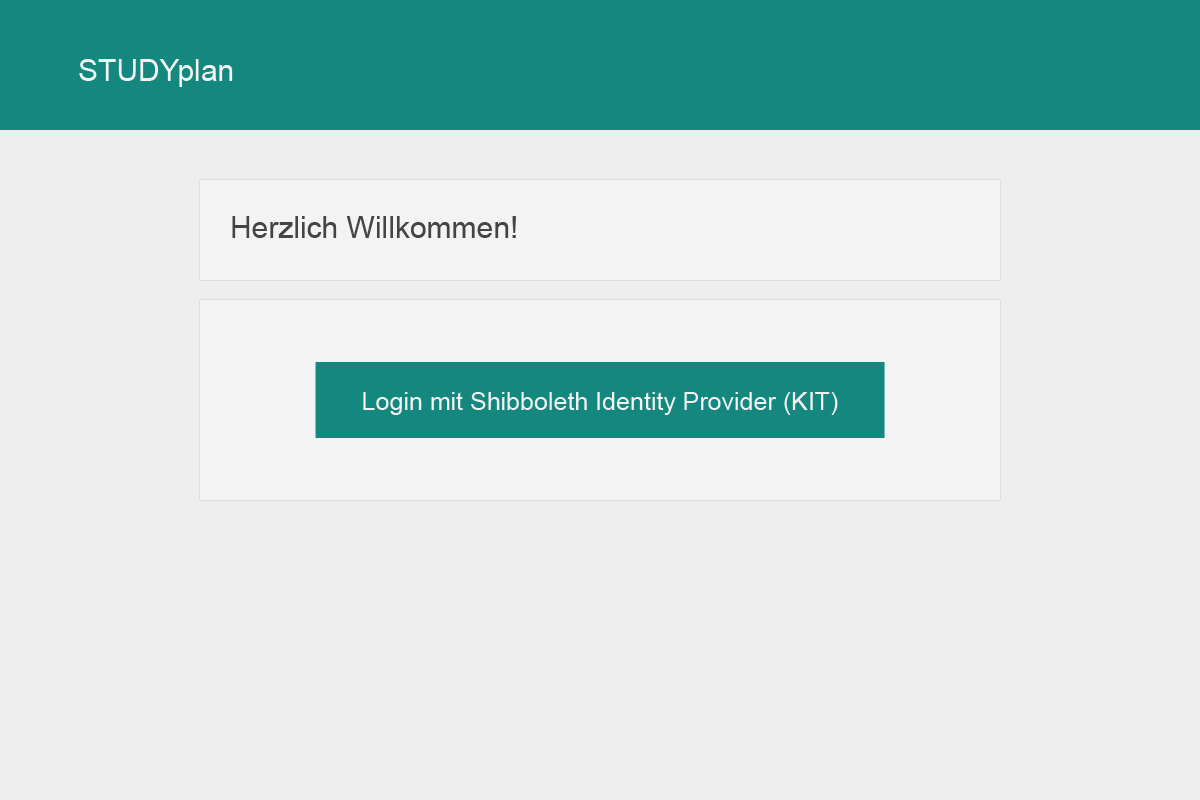
\includegraphics[width=0.8\textwidth]{../GUI/ergebnisse/login-1.png}
\end{figure}
\begin{figure}[!h]
	\caption{Erste Seite des Registrierungs"=\gls{Wizard}s mit Eingabe von Studienfach und Studienbeginn}
	\label{fig:gui-registrierung-1}
	\centering
	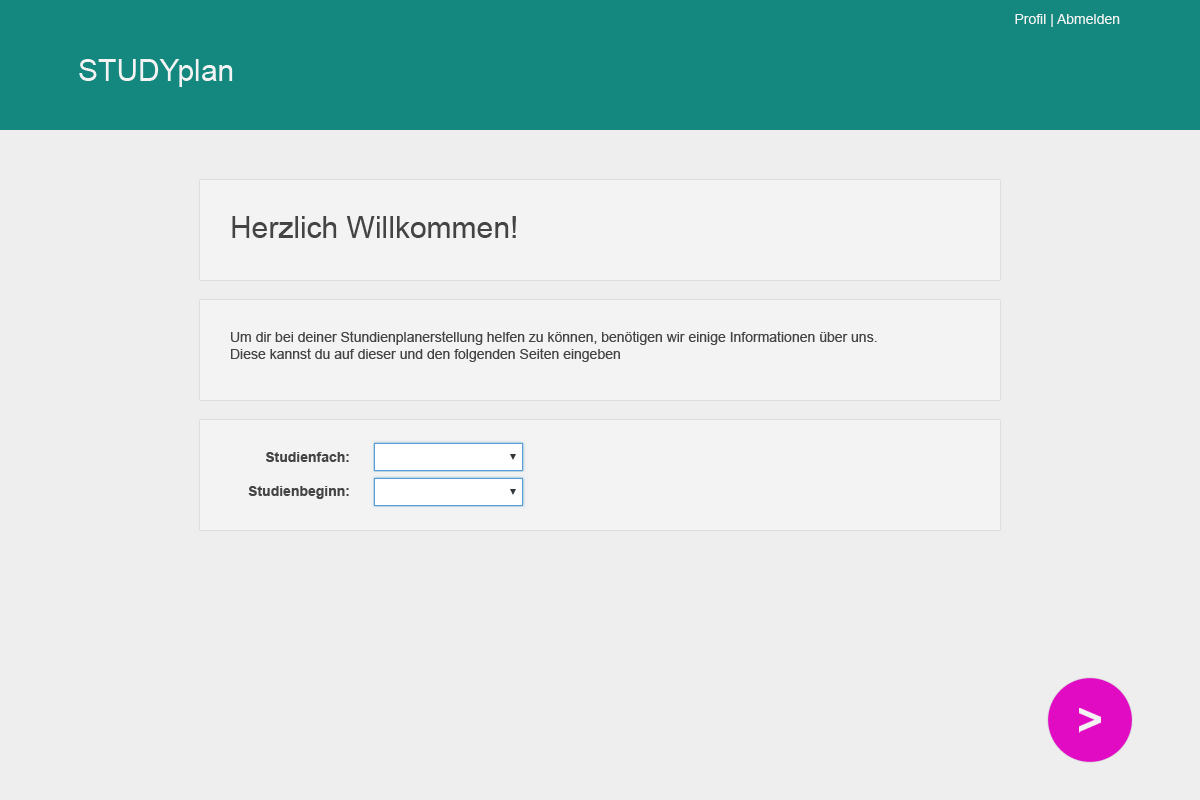
\includegraphics[width=0.8\textwidth]{../GUI/ergebnisse/registrierung-1.png}
\end{figure}

\begin{figure}
	\caption{Zweite Seite des Registrierungs"=\gls{Wizard}s mit Eingabe der schon begonnenen Module}
	\label{fig:gui-registrierung-2}
	\centering
	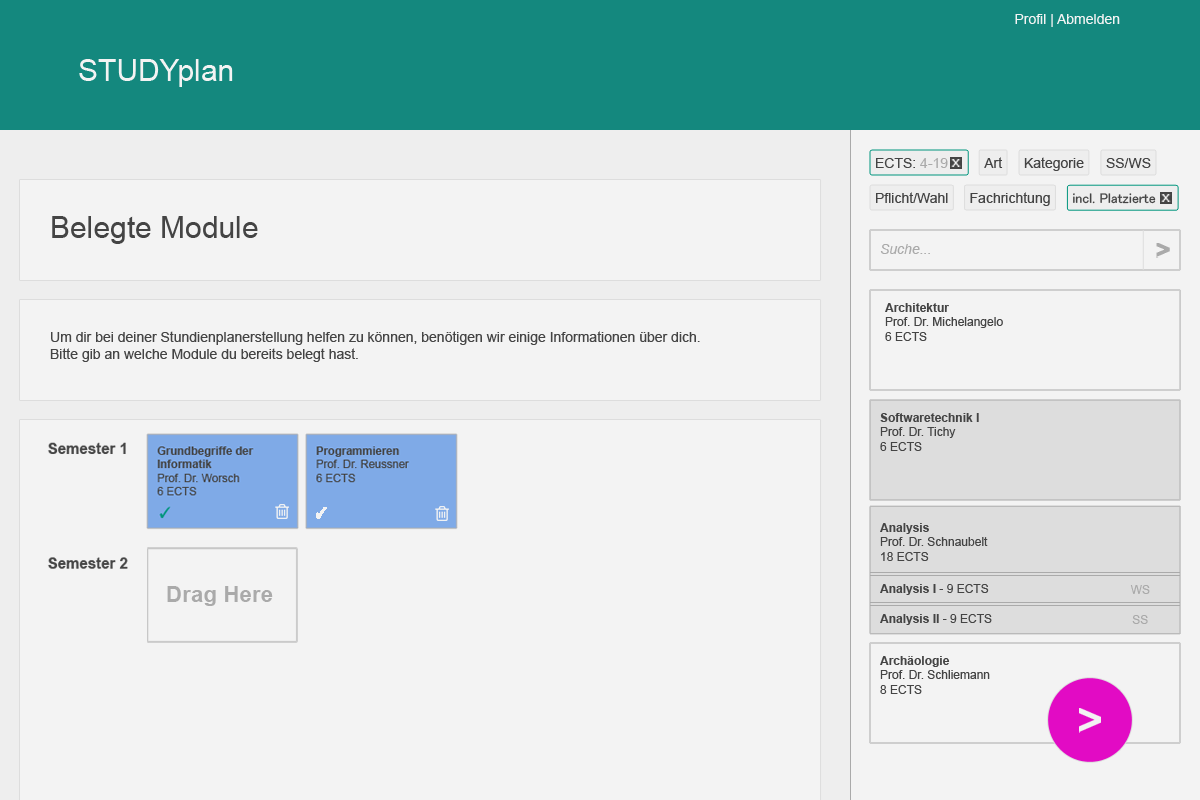
\includegraphics[width=0.9\textwidth]{../GUI/ergebnisse/registrierung-2.png}
\end{figure}

\begin{figure}
	\caption{Hauptseite des Systems}
	\label{fig:gui-hauptseite-1}
	\centering
	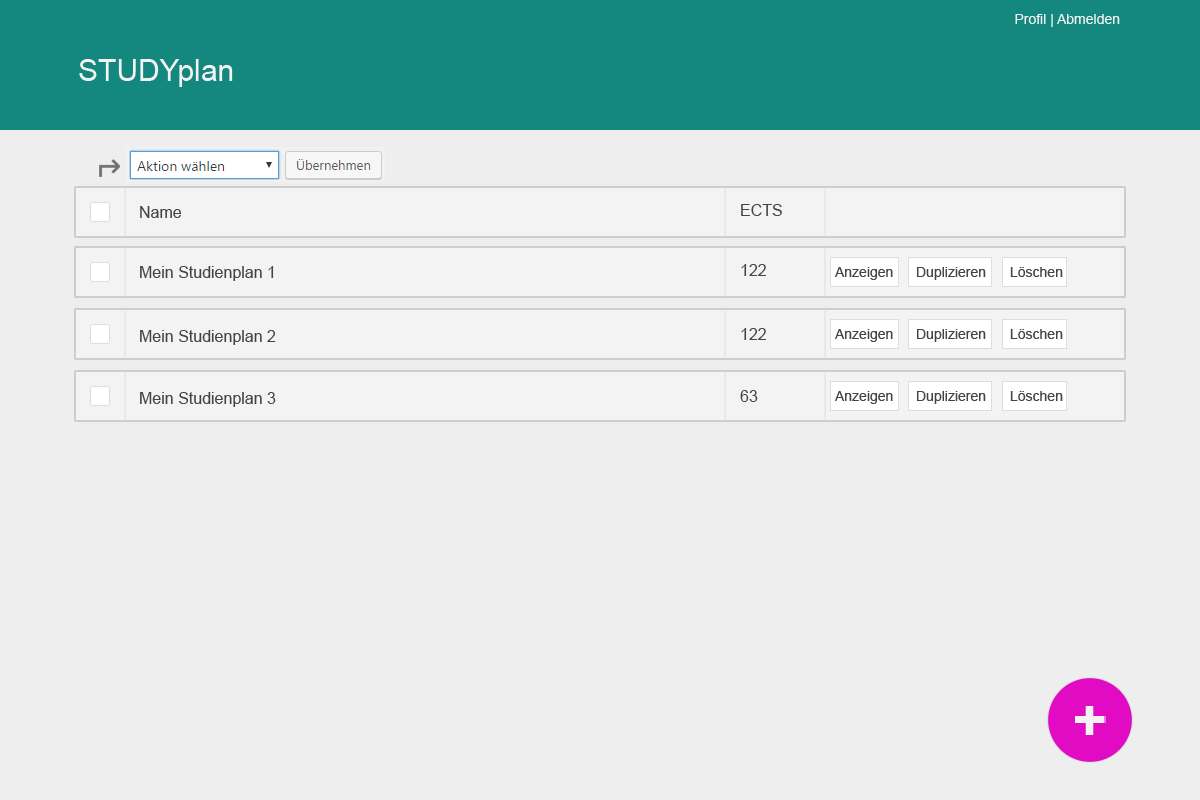
\includegraphics[width=0.9\textwidth]{../GUI/ergebnisse/hauptseite-1.png}
\end{figure}
\begin{figure}
	\caption{Manuelle Bearbeitung des Studienplans}
	\label{fig:gui-bearbeitung-1}
	\centering
	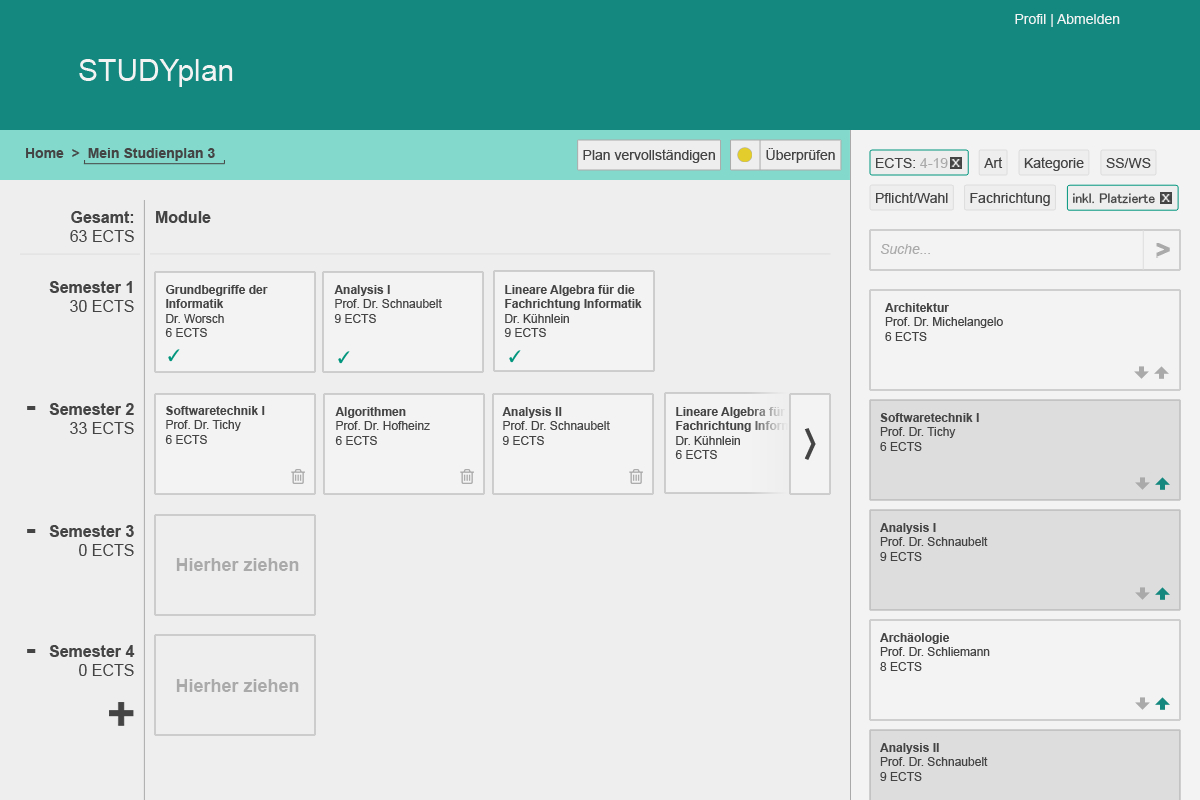
\includegraphics[width=0.9\textwidth]{../GUI/ergebnisse/bearbeitung-1.png}
\end{figure}
\begin{figure}
	\caption{Seitenleiste für Modulfilterung mit offener Kategorie-Auswahl}
	\label{fig:gui-module-filtern-1}
	\centering
	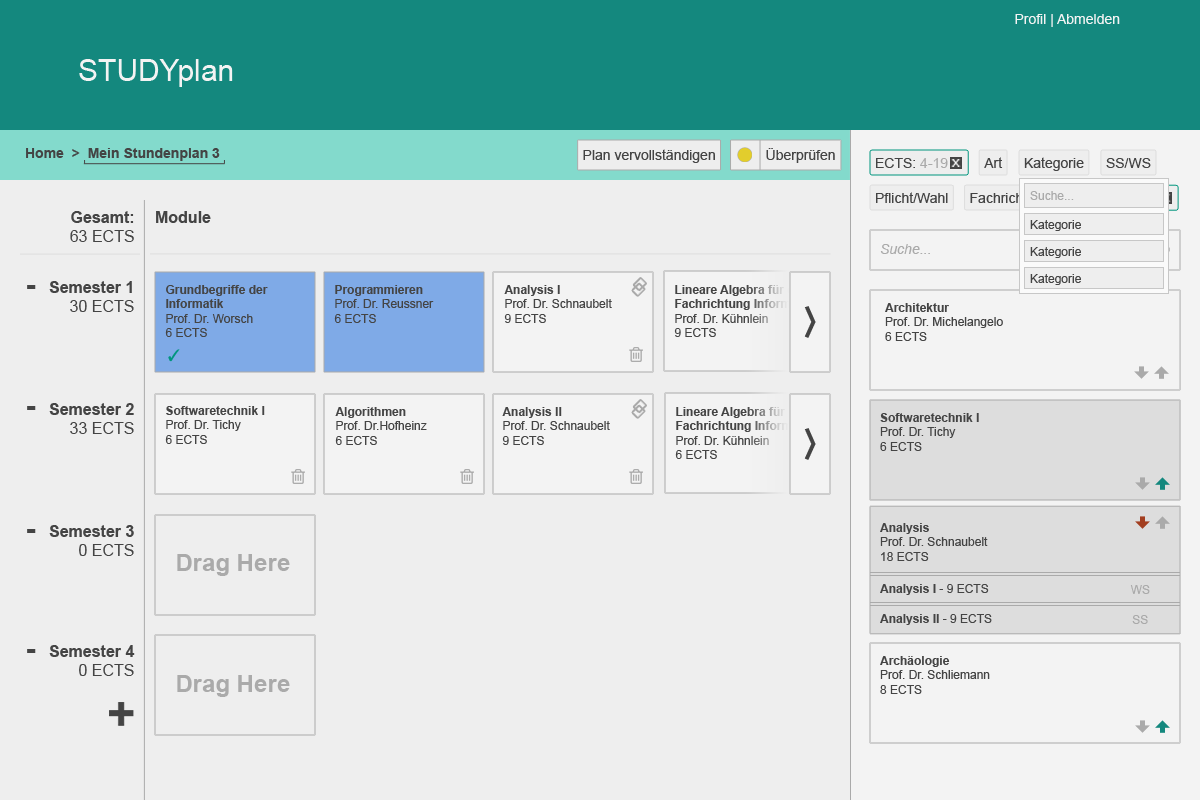
\includegraphics[width=0.9\textwidth]{../GUI/ergebnisse/module-filtern-1.png}
\end{figure}
\begin{figure}
	\caption{Seitenleiste für Modulfilterung mit offener ECTS-Auswahl}
	\label{fig:gui-module-filtern-2}
	\centering
	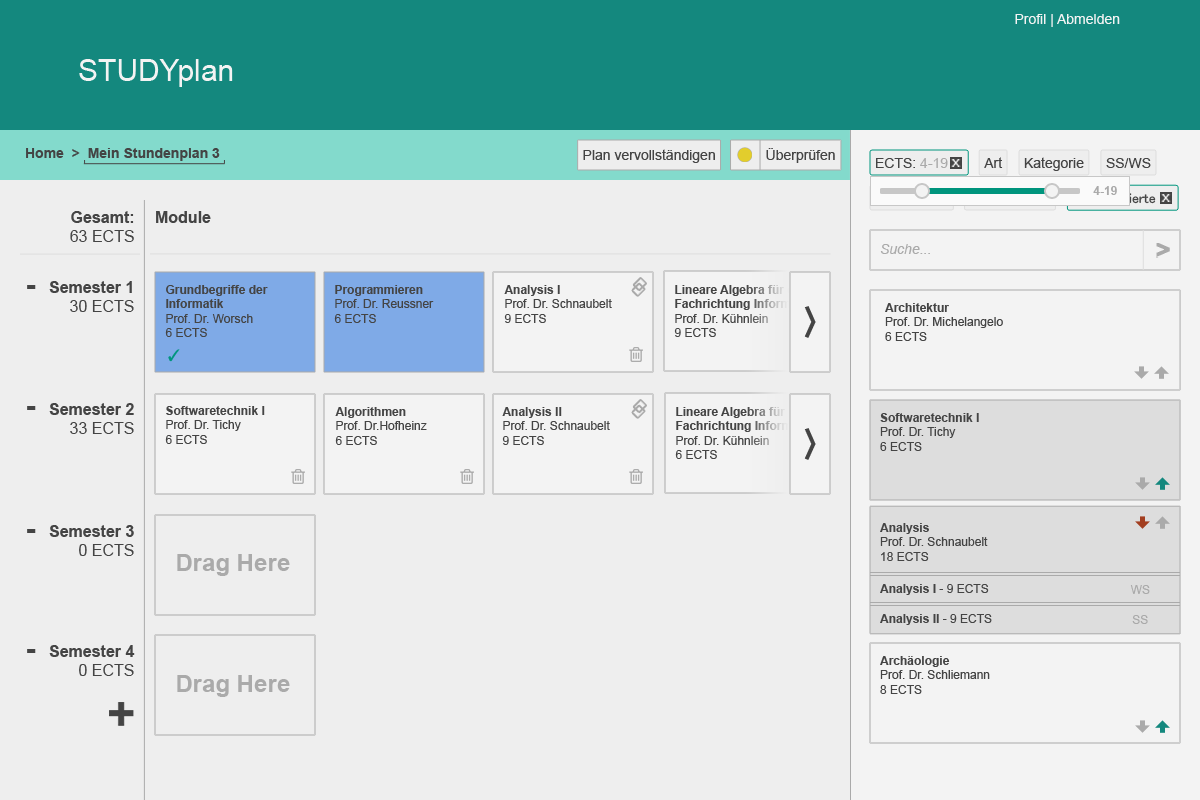
\includegraphics[width=0.9\textwidth]{../GUI/ergebnisse/module-filtern-2.png}
\end{figure}
\begin{figure}
	\caption{Detailansicht für Modul}
	\label{fig:gui-modul-info-1}
	\centering
	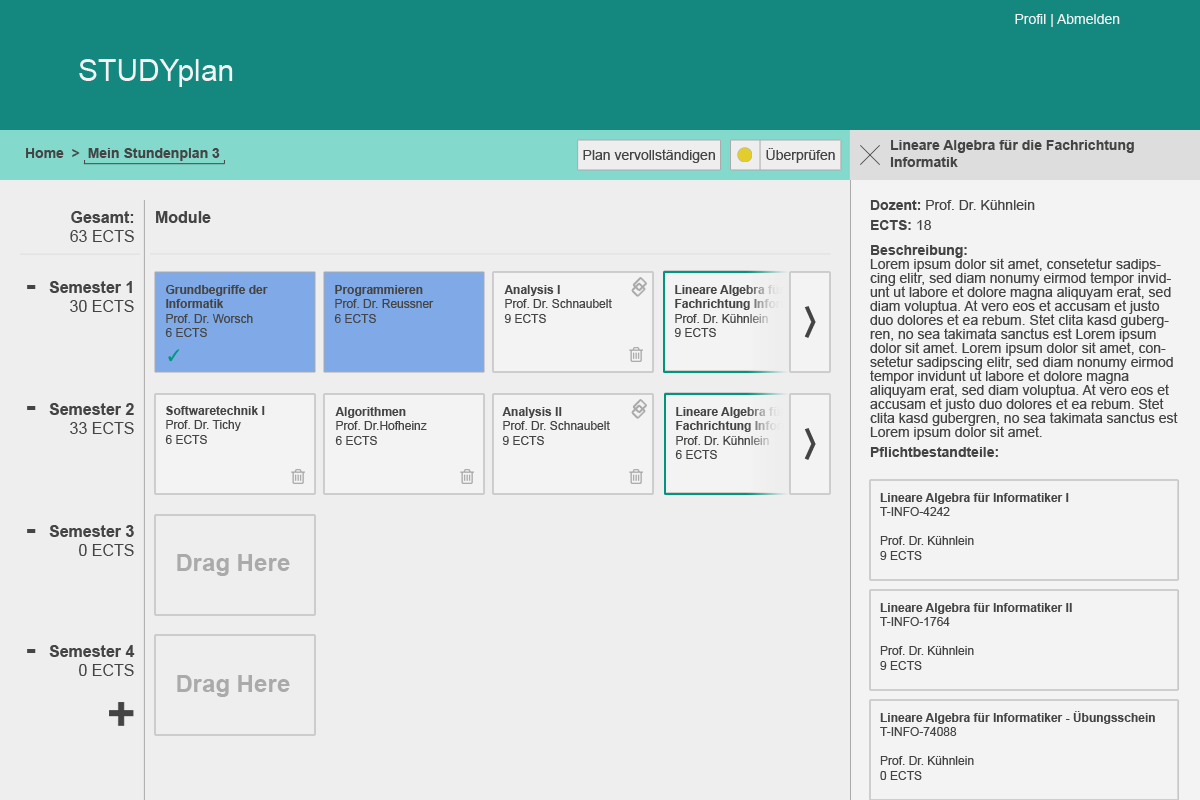
\includegraphics[width=0.9\textwidth]{../GUI/ergebnisse/modul-info-1.png}
\end{figure}
\begin{figure}
	\caption{1. Seite des Generierungs-Wizards}
	\label{fig:gui-generierung-1}
	\centering
	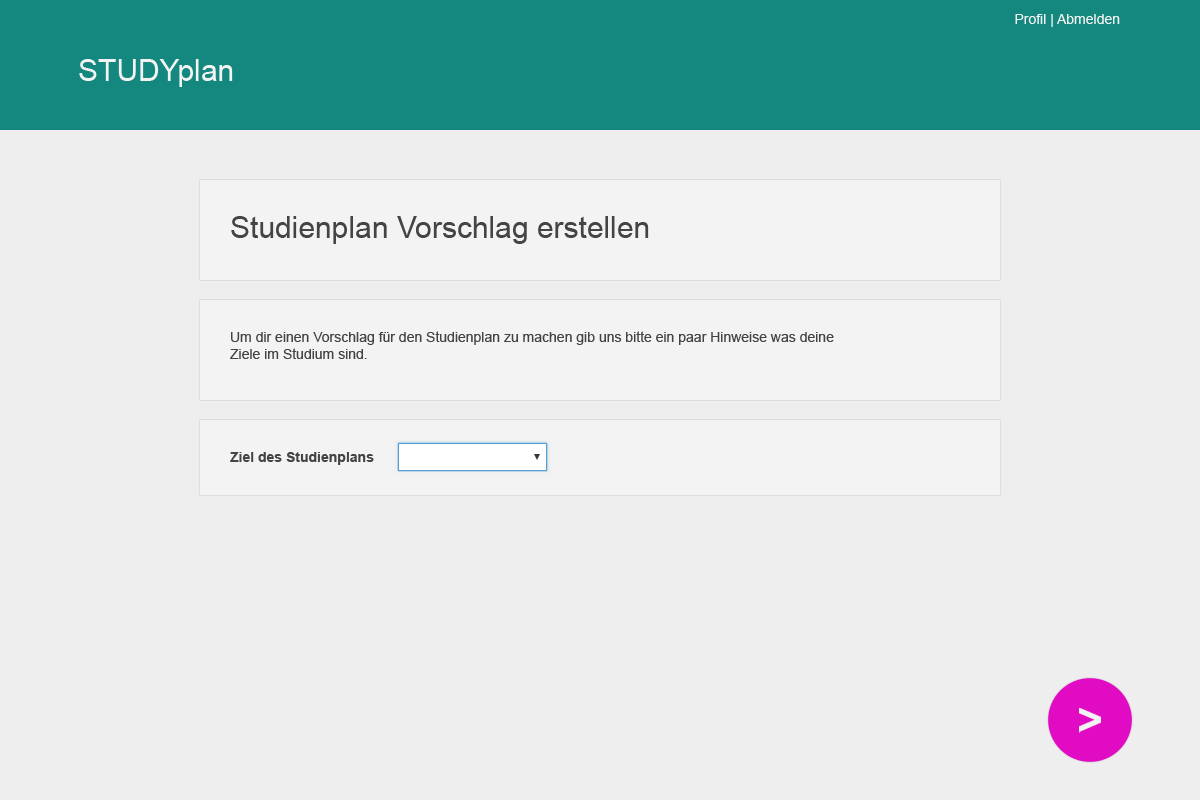
\includegraphics[width=0.9\textwidth]{../GUI/ergebnisse/generierung-1.png}
\end{figure}

\begin{figure}
	\caption{2. Seite des Generierungs-Wizard}
	\label{fig:gui-generierung-2}
	\centering
	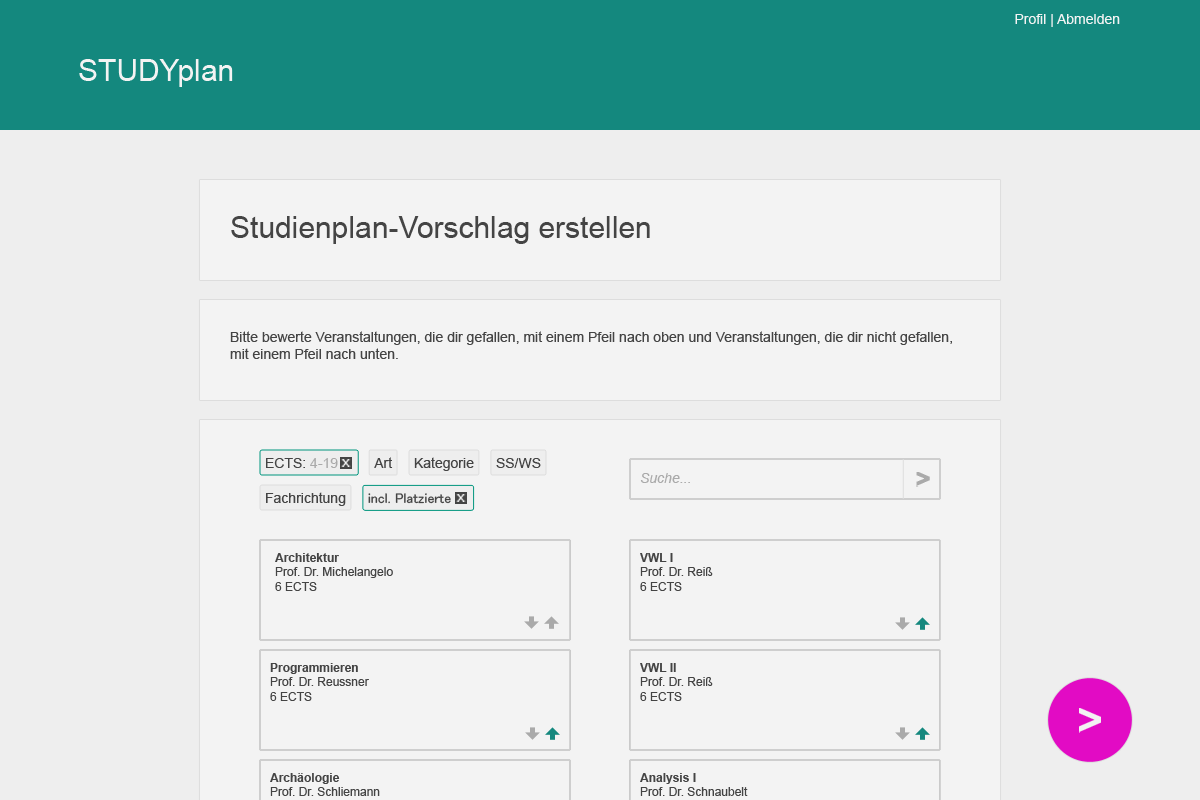
\includegraphics[width=0.9\textwidth]{../GUI/ergebnisse/generierung-2.png}
\end{figure}

\begin{figure}
	\caption{3. Seite des Generierungs-Wizard}
	\label{fig:gui-generierung-3}
	\centering
	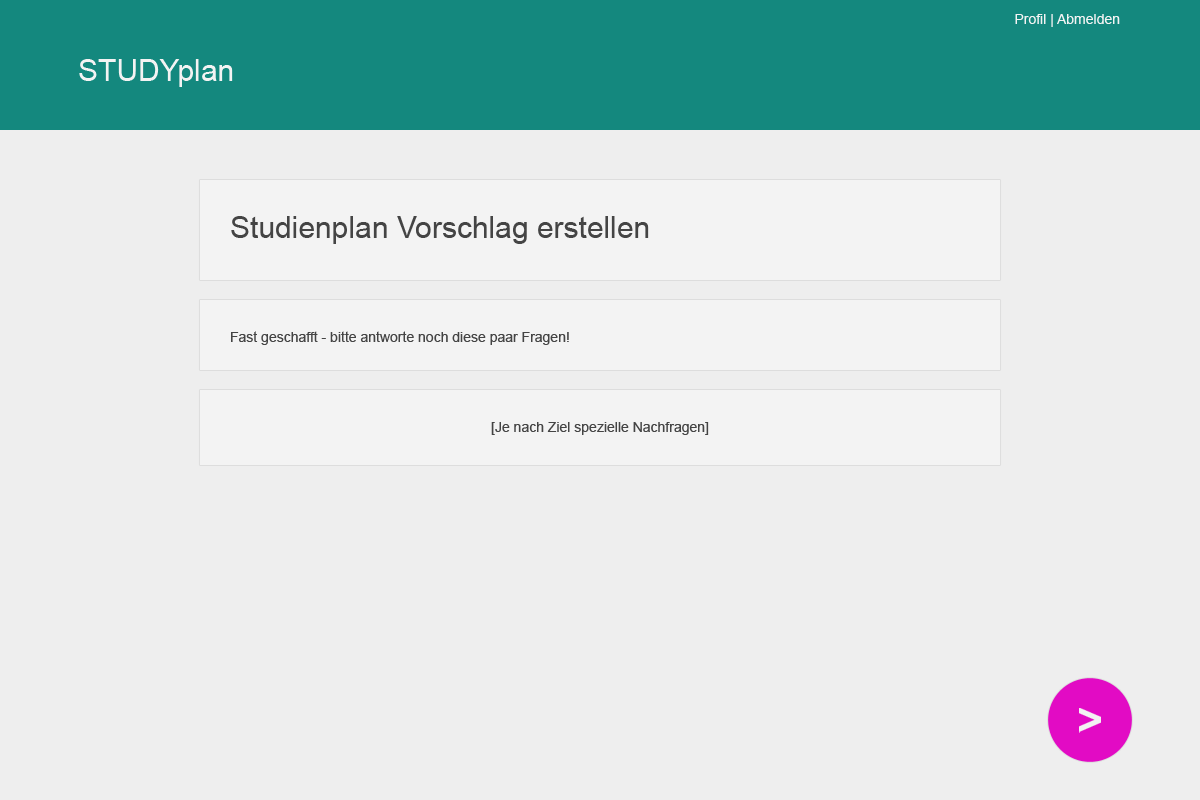
\includegraphics[width=0.9\textwidth]{../GUI/ergebnisse/generierung-3.png}
\end{figure}

\begin{figure}
	\caption{Anzeige des generierten Studienplans}
	\label{fig:gui-generierung-4}
	\centering
	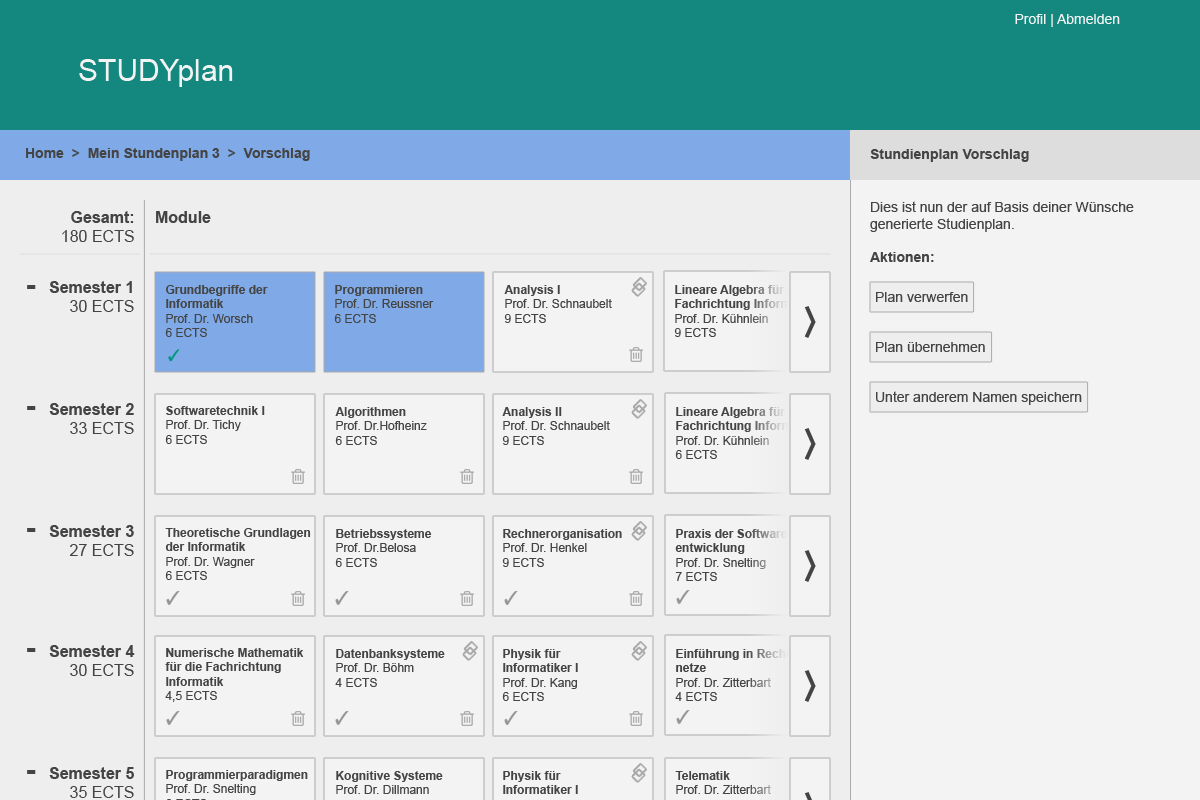
\includegraphics[width=0.9\textwidth]{../GUI/ergebnisse/generierung-4.png}
\end{figure}
\begin{figure}
	\caption{Erfolgreiche Verifizierung}
	\label{fig:gui-verifizierung-1}
	\centering
	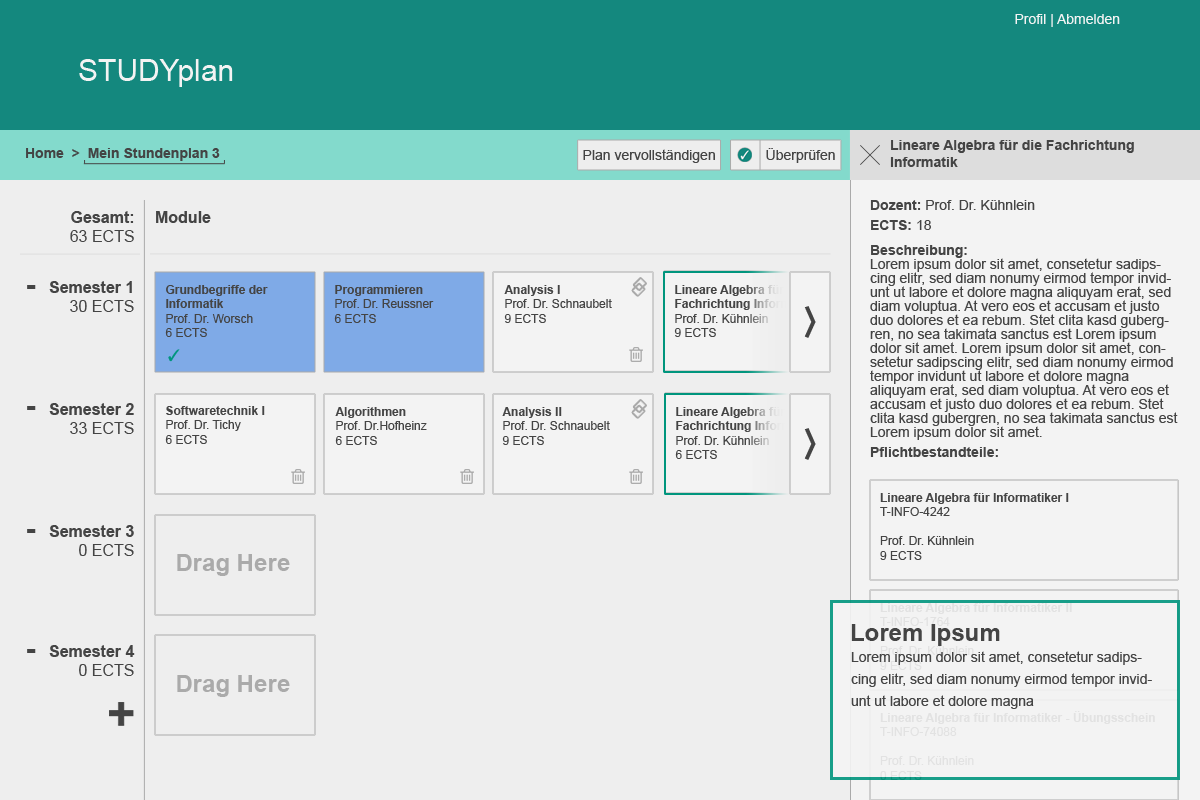
\includegraphics[width=0.9\textwidth]{../GUI/ergebnisse/verifizierung-1.png}
\end{figure}
\begin{figure}
	\caption{Fehlgeschlagene Verifizierung}
	\label{fig:gui-verifizierung-2}
	\centering
	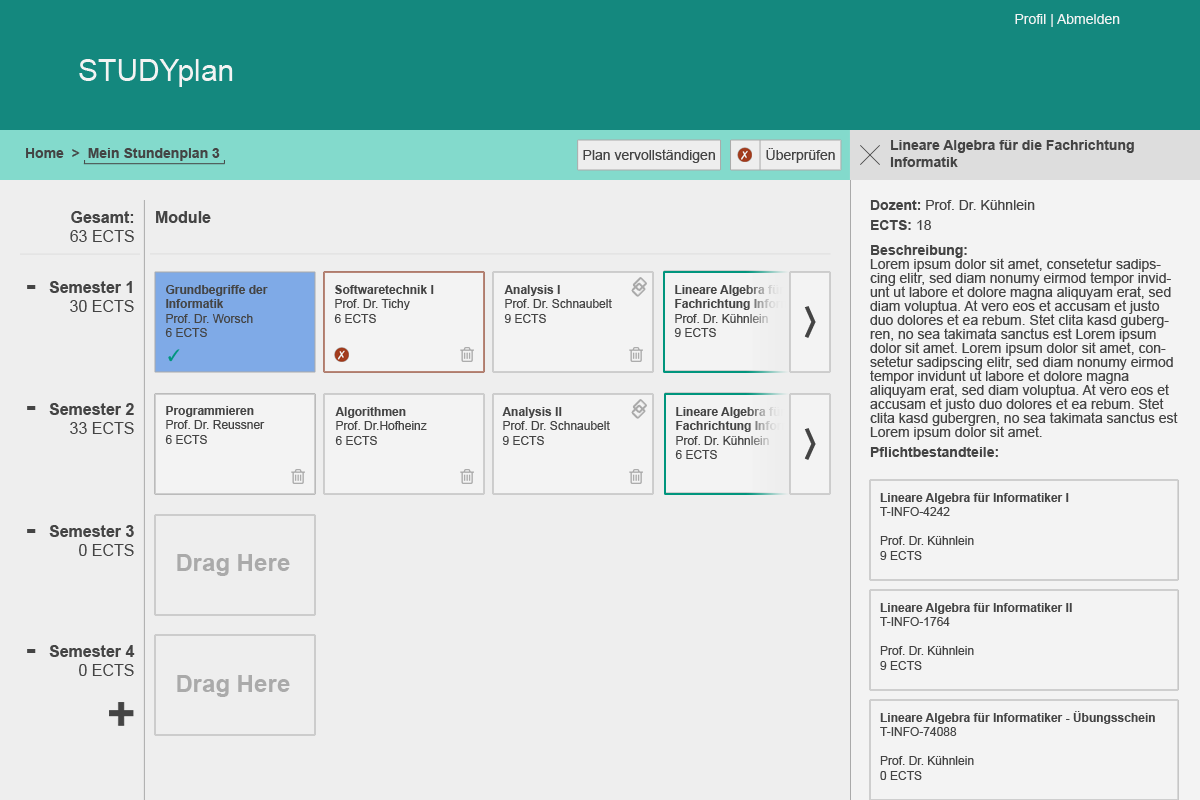
\includegraphics[width=0.9\textwidth]{../GUI/ergebnisse/verifizierung-2.png}
\end{figure}
\begin{figure}
	\caption{Profilansicht}
	\label{fig:gui-profil-1}
	\centering
	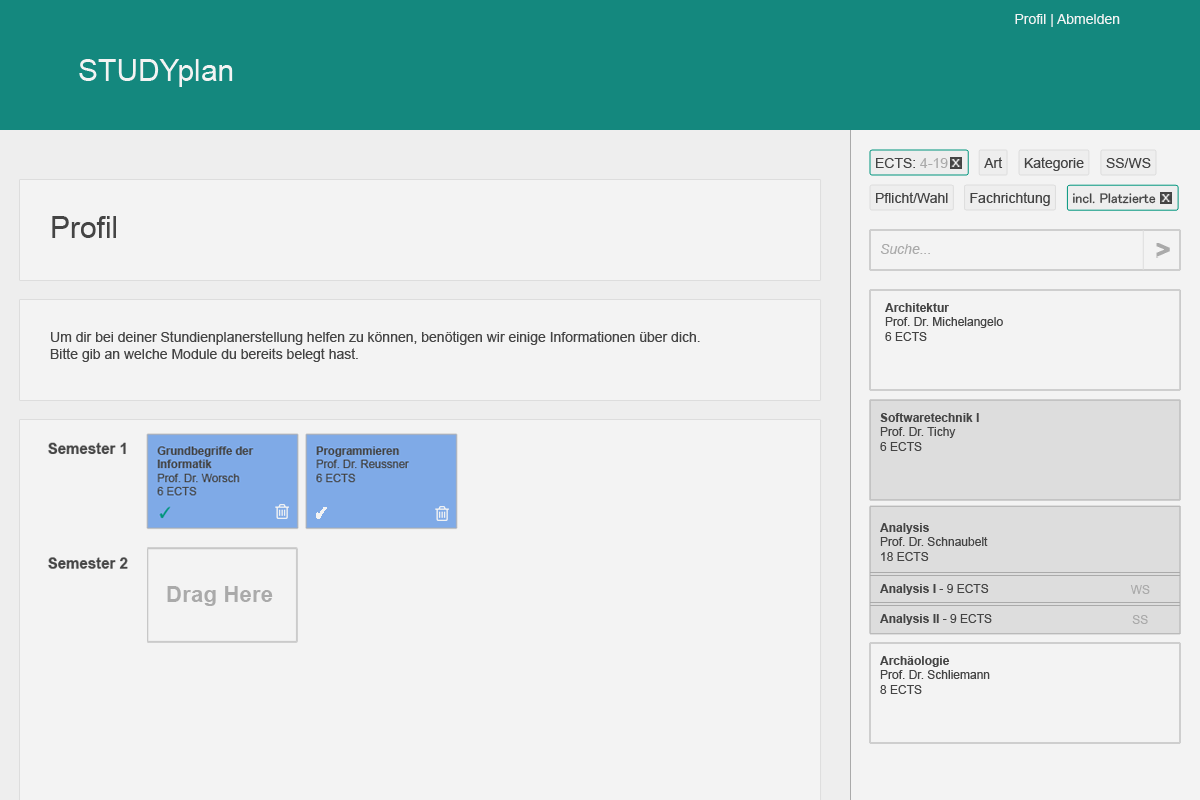
\includegraphics[width=0.9\textwidth]{../GUI/ergebnisse/profil-1.png}
\end{figure}
\FloatBarrier
\end{appendices}
\end{document}
